% --------------------------------------------
%		CAPITOLO 5
%---------------------------------------------

\begin{comment}

Intro should stress: 
1. why the characterizazion of TJMP2 is so important for the upgrade project (OBELIX will have the same matrix analog/readout of TJMP2 + changes in the periphery to implement the trigger logic and memories for application in Belle II)
%2. what we have done in Pisa (see below) 

%3. The chip used in the DESY TestBeam was fully characterized in Pisa: TOT calibration with internal charge injection & with radioactive sources 🡪  important inputs used in TB data reconstruction and in the simulation SW of the upgraded VTX with MAPS
4. Explored also different registers settings to operate the chip with lower THResholds
 	- important after radiation damage to run at low THR to keep the hit efficiency high
5. Discovered & investigated an important issue with cross talk, due to digital signal from the redout, showing up when running the chip with THR below ~ 250 e- 
hot pixel studied to understand which digital signal was responsible & mitigate the effect with different settings/bias



Sections of this chapter could be: 
1. Matrix and flavour
2. Threshold and noise: 
	S curve internal injection, results with TB settings
	Threshold dispersion and tuning 
	Results from measurements done later (Ludovico talk TREDI) 
3. TOT calibration with internal injection 
	Also add the issue with injection circuit but not too much emphasis. 
4. Response to radioactive source and absolute calibration
5. Operation with low threshold 
	Explain the function of the various registers used (see Eleonora thesis, and maybe can 		add also some scope picture). 
	Register optimization 
	Comparison with simulation 
	Can add at the end some nice picture of the optimized thr and tuning 
6. Cross talk issue and mitigation 
	Description of the issue tests done and plans to mitigate it in OBELIX
7. TB JUne 2022 results
	prospettive del TB 2023
\end{comment}

%%%%%DRAWBACK!
%%%%%AFOREMENTIONED
%%%%%SHORTCOMINGS


\chapter{TJ-Monopix 2}

In the previous chapter we have seen the fundamental steps that had lead to the development of the CMOS MAPS sensors thechnology and the history of their many different prototypes. \\
Here we will go through the main features of TJ-Monopix 2, which represents the improvement of its predecessor TJ-Monopix 1, conceived(designed) to address efficiency degradation after irradiation. The characterization of the chip has crucial consequences in the VTX upgrade program and therefore in the evolution of the OBELIX (sensor).\\
The chip W14R12 (\vref{fig:w14r12}) wihch is one of the matrices tested during the Test Beam in Desy (July 2022) has been fully characterize in Pisa and in particular several aspects have been analyzed, among which:

\begin{itemize}
\item TOT calibration by internal charge injection;
\item caracterization with radioactive sources;
\item systematic study of different registers settings in order to operate the chip with lower thresholds;
\item investigation of an important issue with cross talk, due to digital signal from the readout, discovered operating at lower threshold (below 250 $e^{-}$).
\end{itemize}

This well-structured study returned relevant results which have helped in TestBeam data reconstruction and in the simulations SW(???) of the upgraded VTX with CMOS MAPS devices.

%%METTI I TIPI E CHE IL NOSTRO è CZ (SPIEGA NEL QUARTO LE DIFFERENZE)


%This articulate (well-structured) study(analysis) returned relevant (decisive, significant) results which have helped in TestBeam data reconstruction and in the simulations SW(???) of the upgraded VTX with CMOS MAPS devices.



%FOTO TJ MONOPIX 2
\begin{figure}[h!]
\centering
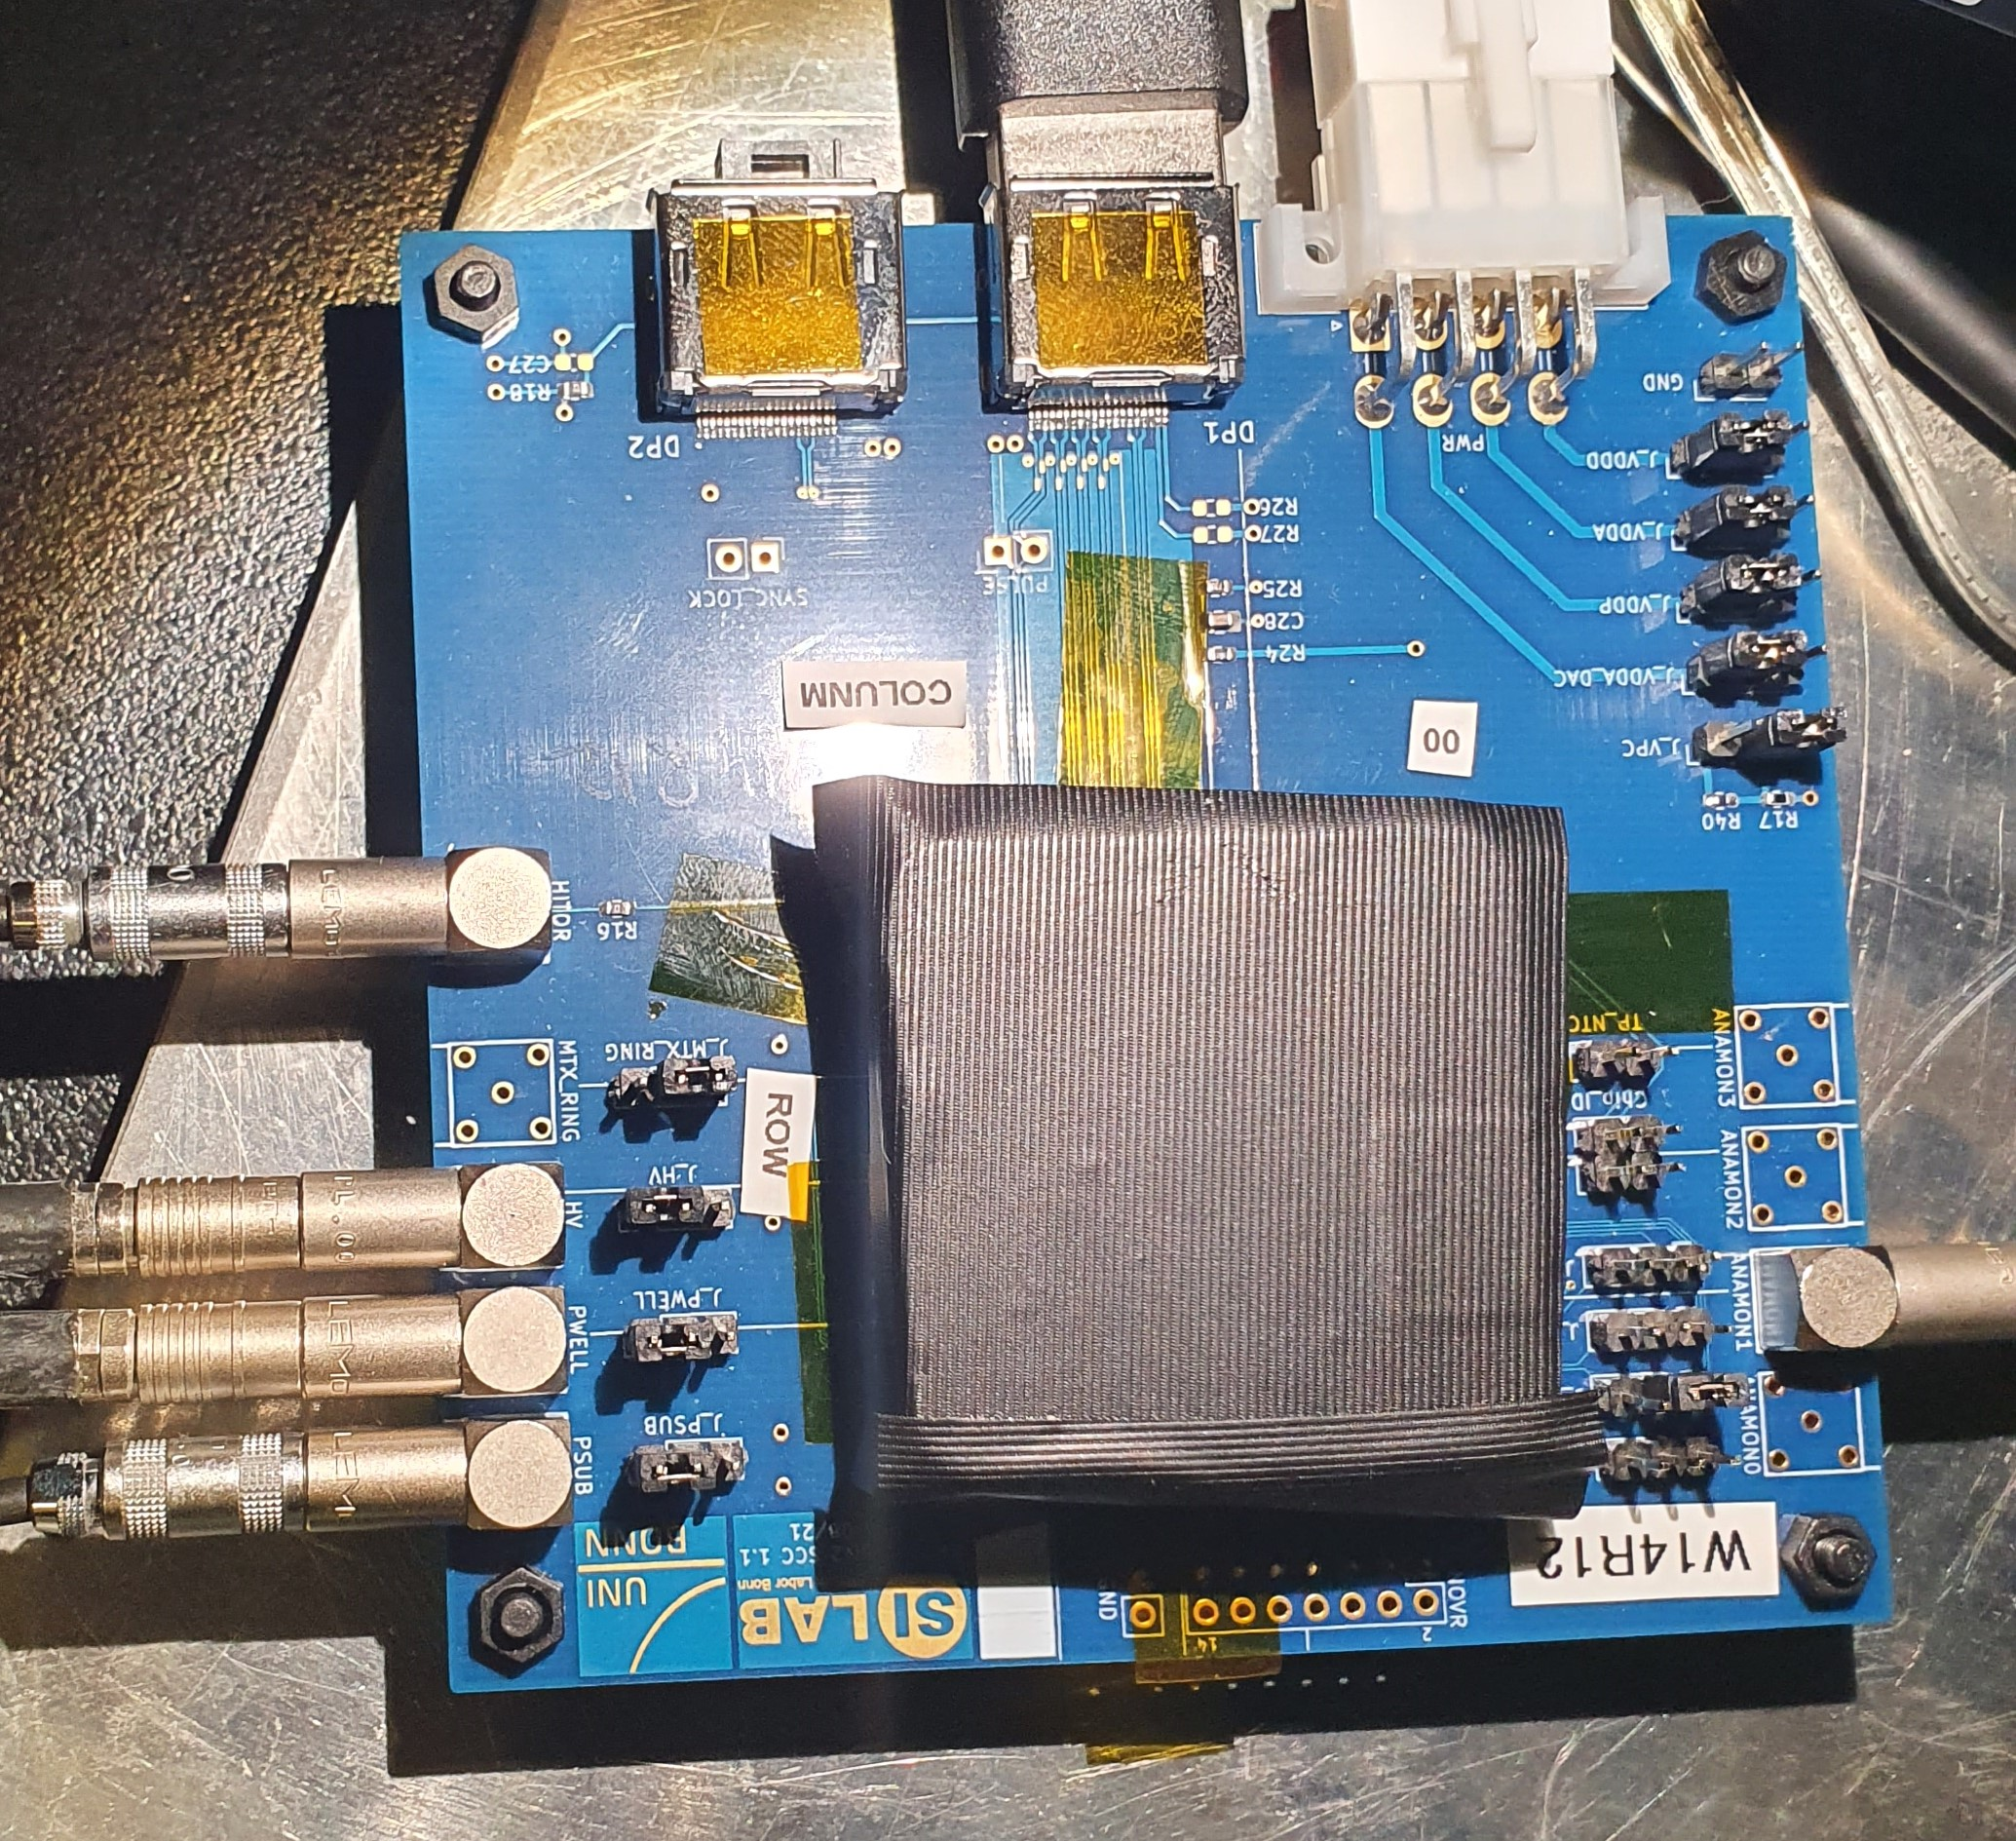
\includegraphics[scale=.08]{W14R12}
\caption{The W14R12 chip tested during the Test Beam in Desy.}
\label{fig:w14r12}
\end{figure}




% --------------------------------------------
%	5.1 MATRIX AND FLAVORS
%---------------------------------------------

\section{Matrix and flavors}

%DEVI SPIEGARE COSA è UGUALE A TJMONOPIX 1 SPIEGATO NEL QUARTO. QUI LE DIFFERENZE E LO STUDIO DELLE CARATTERISTICHE.

Tj-Monopix 2 is the next generation small collection electrode DMAPS prototype in TowerJazz 180 nm. The need to create a sensor capable to mantain high efficiency even after irradiation, required improvements compared to Tj-Monopix 1 in two important fields: a lower operating threshold and different pixel layout to increase charge collection efficiency all over its area, expecially in the corners.\\

To achieve these goals, a different front-end in pixel circuit was implemented and a lot of efforts have been focused on optimizing pixel layout in order to reduce its size which has been decreased to 33.04 x 33.04 $\mu m^{2}$. As a matter of fact we have seen in (REFERENCE) that pixel's diensions are critical to accomplish faster charge collection across all active area, increasing the lateral electric field. For this reason it was necessary a special effort to design and create a smaller pixel but still adequate to embody the full digital readout . All of this required to work at the technology density limit and also further modification at the circuit design, such as single ended data transmission in order to reduce the column-bus width.


%%%RIFERIMENTO AL 4 SULLE implicazioni delle DIMENSIONI.



%-----------------------------------------------------------------------------------------------%

\subsection{Flavors}

The protype is a 2 x 2 $cm^{2}$ pixel matrix which consists of 512x512 pixels and all of them are designed with a reduced deep p-well geometry (RDPW) because as it was demonstrated during the testing of TJ-Monopix1, this type of structure has a superior charge collection properties compared to full deep p-well coverage (FDPW) (figure \vref{fig:tj1pix_cov}). The total active area of the matrix is approximately 286 $mm^{2}$. 

\begin{figure}[h!]
\centering
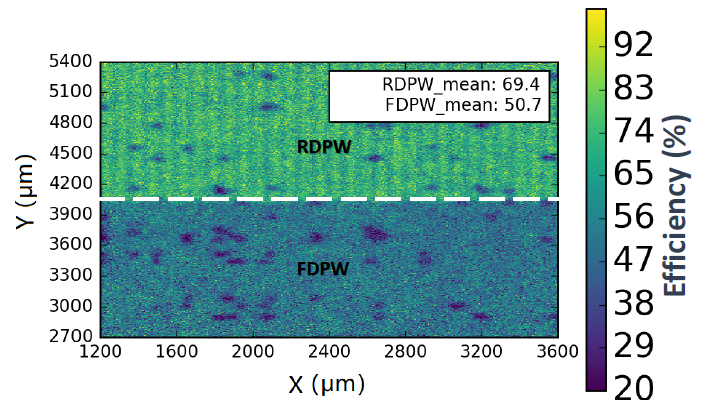
\includegraphics[scale=.6]{Tj1pix_cov}
\caption{Detection efficiency map of a TJ-Monopix1 chip with 25 $mu$m p-epitaxial layer that has been irradiated to $10^{15}$ $n_{\textit{eq}}$/$cm^{2}$ NIEL.}
\label{fig:tj1pix_cov}
\end{figure}

As we can see in figure \vref{fig:tj2matrix}, the matrix is divided in four sectors, named \textbf{flavors} that implement different variation of the front-end circuit. In the first two flavors the collection electrode is DC-coupled directly with the readout electronics,  the continuous baseline reset is implemented by a forward bias diode and they differ for the pre-amplifier circuit design. The second flavor, named \textbf{Cascode FE}, includes an extra cascode transistor that increase the pre-amplifier gain and results in 50\% reduction of the threshold dispersion compared to the first flavor, the \textbf{Normal FE}. The other two flavors consist of AC-coupled pixels (through a metal-oxide-metal MOM capacitor) [with front-side HV biasing] and in particular the \textbf{HV-Cascode FE} also incorporate the aforementioned pre-amplifier variation. AC-coupling allows to apply an high positive bias voltage (HV) to the collection electrode, but at the same time it also causes signal losses mainly due to the additional parasitic capacitance introduced at the sensitive input node.\\
The BCID bus width has been increased  to 7-bits due to higher gain and ToT slope with respect to Tj-Monopix 1. \\
It's worth mentioning here that the large column height (approx. 17 mm) due to large matrix area and the aggressive column-bus routing (which refers to the minimum line width and spacing) because of the smaller pixel size (always with respect to TJ-Monopix 1) generated a significant signal transmission delay due to the RC low pass filtering effect of the long metal wires. Consequently a special circuit has been planned(designed) that adds a variable delay to the hit pulse across the column that matches that of the BCID signal.



%%%PERIPHERY PAG 138


\begin{figure}[h!]
\centering
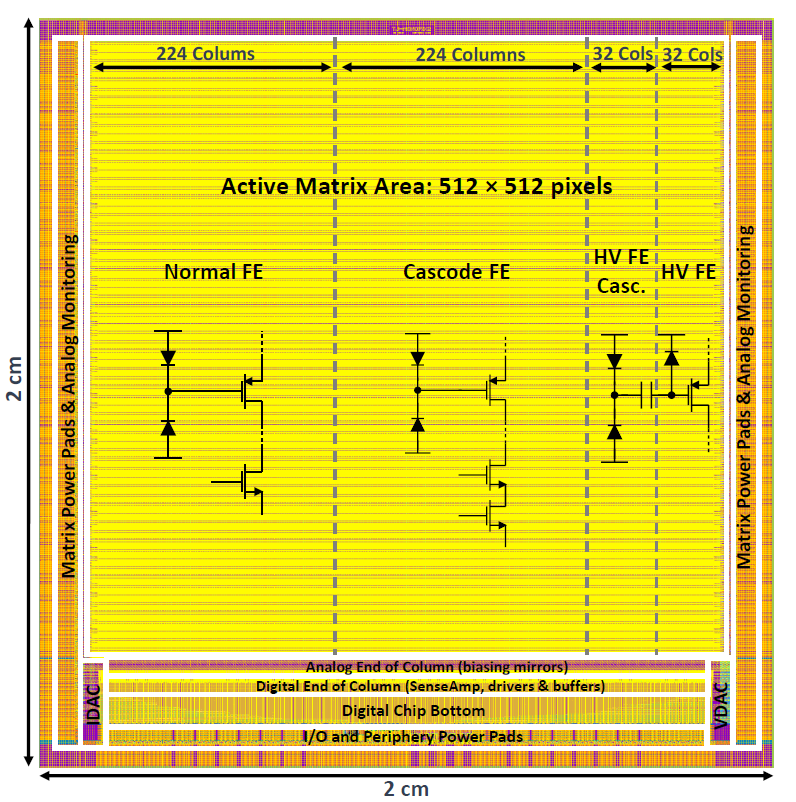
\includegraphics[scale=.5]{Matrix}
\caption{The layout of the TJ-Monopix2 prototype divided in four different flavors: \textbf{Normal}, \textbf{Cascode}, \textbf{HV-Cascode} and \textbf{HV FE}.}
\label{fig:tj2matrix}
\end{figure}


%-----------------------------------------------------------------------------------------------%

\subsection{Pixel design}

VEDI\\ 

The 2 x 2 pixel core layout, shown in figure \vref{tj2core} is fully optimized and is designed in order to share as much functionality as possible between the four pixels. The analog area incorporate the front-end circuit, the 3-bit threshold tuning DAC and the pixel configuration registers. The digital region is composed by the 7-bit LE and TE memory (14 SRAM cells per pixel), the 10 bit address ROM (2 bit for the pixel position inside the core and 8 for the group address), the readout control logic and the hit delay circuit that is used to correct for the BCID propagation delay. Two different token signal are used to set the priority of the pixels during the readout: the fast one that propagates across the double column estabilished the priority between the cores and the local one, which arbitrates the reading order of the four pixels inside each core.

\begin{figure}[h!]
\centering
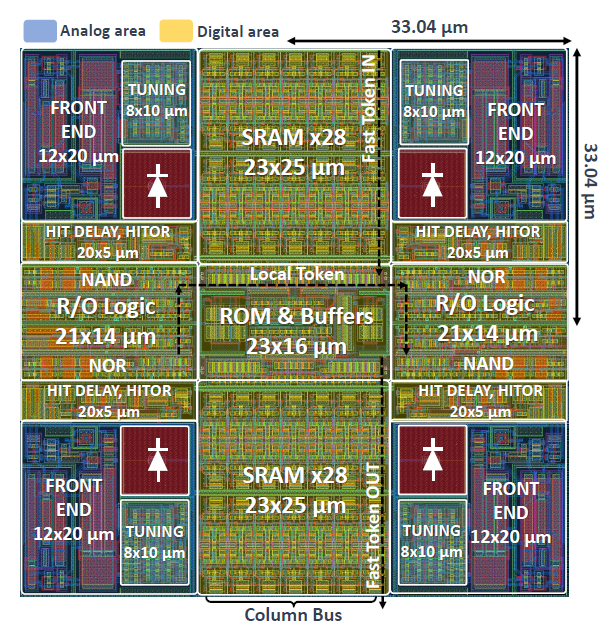
\includegraphics[scale=.5]{pixel_core}
\caption{Layout of a TJ-Monopix 2 2x2 pixel core. In blue the analog area and in yellow the digital one.}
\label{fig:tj2core}
\end{figure}


%-----------------------------------------------------------------------------------------------%

\subsubsection{Improved front-end circuit design}

As we have seen above, there are two variations of the front-end circuit,  ''normal'' and ''cascode'' type. The latter in particular includes an extra cascode transistor which increases the pre-amplifier gain and consequently reduces the threshold dispersion.\\
Moreover in TJ-Monopix 2 it was preferred to incorporate a simple diode to reset the input node instead of a PMOS transistor, which was the techonology implemented in TJ- Monopix 1. A side effect of this choice is that the relationship between charge injected and the ToT of the detected signal is not linear anymore, because the diode is a not linear element and its discharge rate also depends on the collected charge. Indeed in the following analysis it was necessary to fit the ToT trend with a more complex function. But at the same time, the advantages are its simplicity ($p^{+}$ diffusion within the n-well collection electrode) and also the fact that it allows to increase radiation tolerance to TID effects, which was one of the key working area in the upgrade of the sensor, in order to design a final(conclusive) prototype to employ in the experiments subjected to high radiation doses.[pag 153???] \\


In the last two AC-coupled flavors are implemented the same improvements, but here the different coupling provokes an important loss in the collected charge, as verified during the testing phase of TJ-Monopix 1 (50\% losses), due at most to additional parassitic capacitances. Thus (THerefore) a lot of (many) efforts have been made to improve this aspect, working on the coupling capacitor values. It is reach a signal loss of 41.5\%, which is an enhancement(progress) with respect to the predecessor.




% --------------------------------------------
%	5.2 THRESHOLD AND NOISE
%---------------------------------------------

\section{Threshold and noise}

In order to achieve the absolute calibration of the whole matrix, the response of each pixel has been characterize by means of the internal charge injection. \\
?????\\
The hit injection circuit included in TJ-Monopix 2 is similar to the one of TJ-Monopix 1, shown in figure(????). It allows to inject artificial hits through an injection capacitance \textbf{$C_{inj}$} connected at the collection electrode, which is equal to 230 aF for both the DC and AC coupling FE. The injected charge is almost linear with the injection pulse amplitude (set by the two registers ''\textbf{$V_{L}$}'' and ''\textbf{$V_{H}$}'', like $\Delta V_{inj}$ = \textbf{$V_{H}-V_{L}$}). Moreover the injection step is finer compare to the one of TJ1 because of the higher voltage DAC resolution, in fact LSB (\textit{Least Significatn Bit})=7.03 mV. The injected charge $Q_{inj}$ can be calculated from:

\begin{equation}
\small
Q_{inj} = \frac{230 \, aF}{q_{{e}^{-}}} \cdot \Delta V_{inj} = 1.4375 \frac{e^{-}}{mV} \cdot 7.03 \frac{mV}{DAC \, unit} \approx 10.1 \frac{e^{-}}{DAC \, unit}  
\end{equation}

Eventually this value has been used to convert the information of the injected charge from DAC unit to electrons unit useful for further analysis.
\\
The four flavors have been separatly analyzed to be able to study their main difference concerning their performance and features, but the same method, called \textit{s-curve method}, explained below has been used. 


%--------------------------------------------------------------------
\subsection{S-Curve method}

In order to obtain the thresold and noise values for all pixels, each one of them has to be injected an arbitrary number of times (100 times in this work) for each value of the injection pulse between a minimum voltage (value), chosen setting the chip register ''\textbf{VL}'' and a maximum volatge (value) set by the ''\textbf{VH}'' register, with a step of 1 DAC unit this is also adjustable). These two levels are provided by the voltage DAC.

So for each injection pulse height, the mean of 100 injection output are considered and it represents one data in the plot.  In this way plotting the average number of detected hits in function of the injected charge, the typical curve better known as ''\textit{S-curve}'' is reconstructed. It can be fit with the \textit{Cumulative Distribution Function (CDF)}:

\begin{equation}
 CDF(Q) = \frac{1}{2} \cdot \bigg(1 + \textit{erf}\bigg(\frac{Q-\mu}{\sigma \sqrt{2}}\bigg)\bigg)
\end{equation}

from which the value of the threshold is evaluated considering the value of the injected charge at half of the curve's maximum height, so the parameter $\mu$ obtained from the fit and the noise instead is evaluated from the fit parameter $\sigma$. \textit{erf(x)} is the Gauss error function. 

Specifically plotting the number of hits observed on each pixel divided by the total number of injections, for each injected charge, the half height corresponds to a charge value for which the pixel detects 50 hits of 100 injected and so when it has an occupancy of 0.5. In figure \vref{ex_scurve} is shown an example.

%%%%SPIEGARE METODO DI LUDOVICO???? 


\begin{figure}
\centering
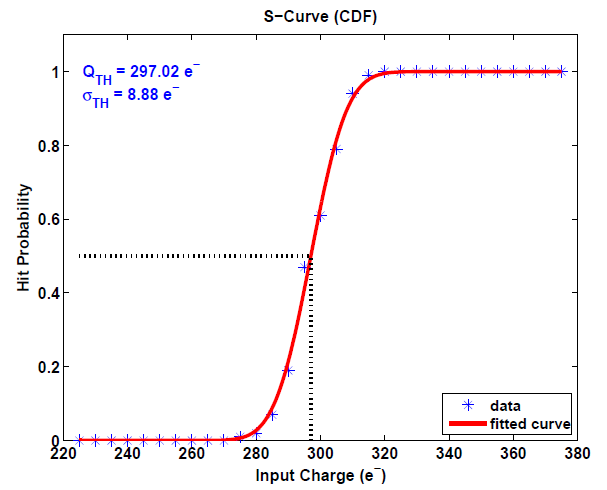
\includegraphics[scale=.7]{scurve_ex}
\caption{An example of the S-Curve fitted by the CDF to evaluate threshold and noise.}
\label{ex_scurve}
\end{figure}

In the following are reported the results of this study for the flavors of all matrix.


\subsubsection{Normal FE}

The first flavor of the matrix is the \textbf{Normal FE}, which consist of 512 rows and 224 columns for a total of 114.688 pixels. The chip registers have been set with the same values used during the Test Beam at Desy (July 2022) which are known as ''\textbf{GOE settings}'' and reported in table \vref{tab:tb_settings}.


\begin{table}[h!]
\centering
\begin{tabular}{>{\columncolor{ProcessBlue!60}} C{3.5cm}|C{3.5cm}}
\rowcolor{lightgray}
Registri & Default Settings (''GOE'') [DAC unit]\\[2ex]
\hline
$I_{THR}$ & 64 \\[0.5ex]
\hline
$I_{BIAS}$ & 50 \\
\hline
$V_{RESET}$ & 143 \\
\hline
$I_{CASN}$ & 0 \\
\hline
$V_{CASP}$ & 93 \\
\hline
$V_{CASC}$ & 228 \\
\hline
$I_{DB}$ & 100 \\
\hline
$I_{TUNE}$ & 53 \\
\hline
$V_{CLIP}$ & 255 \\
\hline
$I_{COMP}$ & 80 \\
\hline
$I_{DEL}$ & 88 \\
\hline
$I_{RAM}$ & 50 \\
\hline
\end{tabular}
\caption{Settings of the main registers used for the W14R12 chip, for Normal and Cascode flavors, during the Test Beam in Desy.}
\label{tab:tb_settings}
\end{table}


\begin{figure}[h!]
\centering
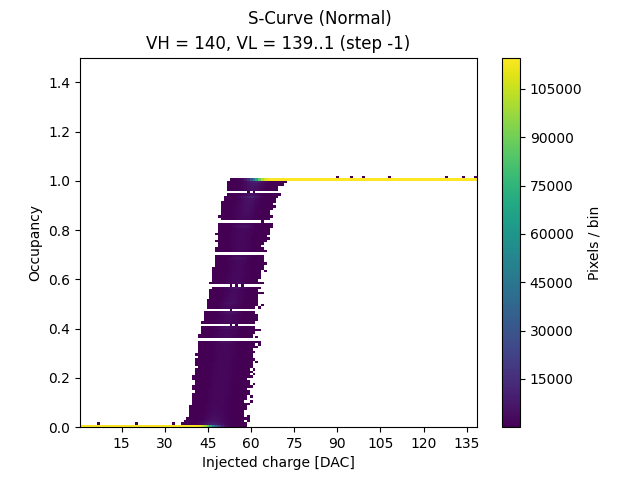
\includegraphics[scale=.6]{all_norm_thscan_140}
\caption{S-curves of all pixels of the Normal FE with an injection pulse of 140 DAC.}
\label{fig:norm_scurve_140}
\end{figure}

Using this setting, none of the pixels were noisy and so it wasn't necessary to use any mask.
In figure \vref{fig:norm_scurve_140} are plotted all the s-curves of the all well-functioning Normal flavor pixels. The width of the plot is a first indication (manifestation, symptom) of the threshold dispersion of the whole flavor.\\

The threshold distribution obtained injecting all pixels as explained above, have been fitted with a gaussian distribution and they are shown in figure \pageref{fig:thdist_norm}.

\begin{figure}[h!]
\centering
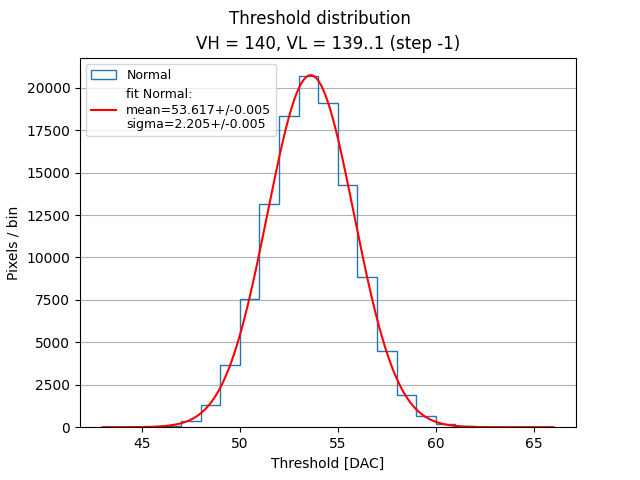
\includegraphics[scale=0.6]{all_norm_thdist_140}
\caption{Threshold distributions of \textbf{Normal} flavor for VH = 140 DAC}
\label{fig:thdist_norm}
\end{figure}


\subsubsection{Cascode FE}

\textbf{Cascode FE} is the second flavor and like \textbf{Normal FE} it consists of 512 rows and 224 columns for a number of total pixels equal to 114.688. For this flavor the same procedure of Normale FE has been followed and also the same values' registers (table \vref{tab:tb_settings}) have been used. There were not find noisy pixels. 
In figure \vref{fig:casc_curve140} the S-curves of all pixels are shown.

\begin{figure}[h!]
\centering
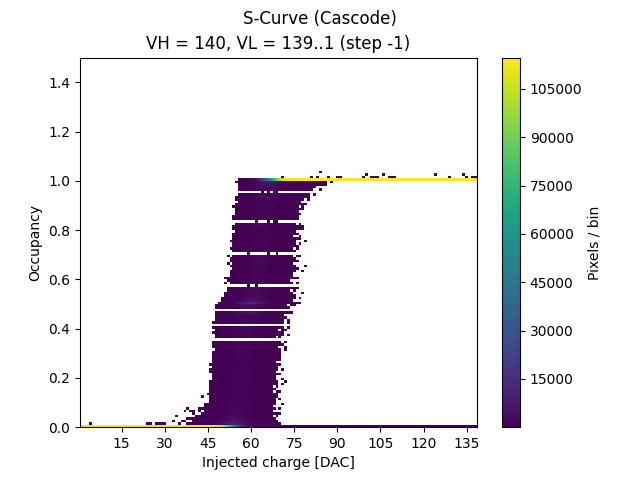
\includegraphics[scale=.5]{all_casc_thscan_140}
\caption{S-curves of all pixels in the \textbf{Cascode} flavor with an injection pulse of 140 DAC.}
\label{fig:casc_scurve140}
\end{figure}

The fit of the threshold distributions instead, are shown in figure \vref{fig:thdist_casc}.

\begin{figure}[h!]
\centering
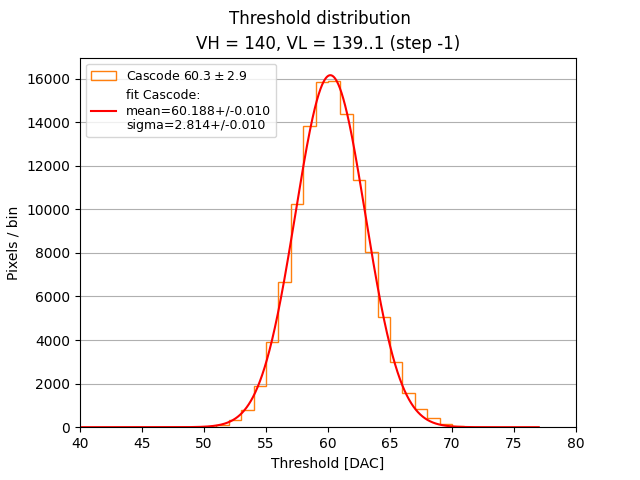
\includegraphics[scale=0.5]{all_casc_thdist_140}
\caption{Threshold distributions of \textbf{Cascode} flavor for VH = 140 DAC.}
\label{fig:thdist_casc}
\end{figure}


\subsubsection{HV-Cascode FE}

The third flavor is \textbf{HV-Cascode FE} where HV stands for \textbf{High Voltage} and it is formed (counts) of 512 rows and 32 columns for a total number of pixel equal to 16384. Also for these last two flavors, the main chip registers are set with the same values tested and used during the Test Beam (@Desy) (but different from those used for the first two flavors). They are reported in table \vpageref{tab:tb_hv_settings} .


\begin{table}[h!]
\centering
\begin{tabular}{>{\columncolor{Green!60}} C{3.5cm}|C{3.5cm}}
\rowcolor{lightgray}
Registri & Default Settings (''GOE'') [DAC unit]\\
\hline
$I_{THR}$ & 30 \\
\hline
$I_{BIAS}$ & 60 \\
\hline
$V_{RESET}$ & 100 \\
\hline
$I_{CASN}$ & 8 \\
\hline
$V_{CASP}$ & 40 \\
\hline
$V_{CASC}$ & 228 \\
\hline
$I_{DB}$ & 100 \\
\hline
$I_{TUNE}$ & 53 \\
\hline
$V_{CLIP}$ & 255 \\
\hline
$I_{COMP}$ & 80 \\
\hline
$I_{DEL}$ & 88 \\
\hline
$I_{RAM}$ & 50 \\
\hline
\end{tabular}
\caption{Settings of the main registers used for the W14R12 chip, for the HV's flavors, during the Test Beam in Desy.}
\label{tab:tb_hv_settings}
\end{table}

As we can see from the plot of the alle S-curves in figure \vref{fig:hvc_scurve_140}, there were a lot of noisy pixels with these choices of values' registers, but at this stage of measurements they were not masked.
As a matter of fact along the y-axis of this plot is displayed the occupancy and when this values becomes higher than 1, it means that the pixel detects more hits than the injected ones, so it could be identified as ''\textit{noisy pixel} (because it results active regardless of the charge injection)''.


\begin{figure}[h!]
\centering
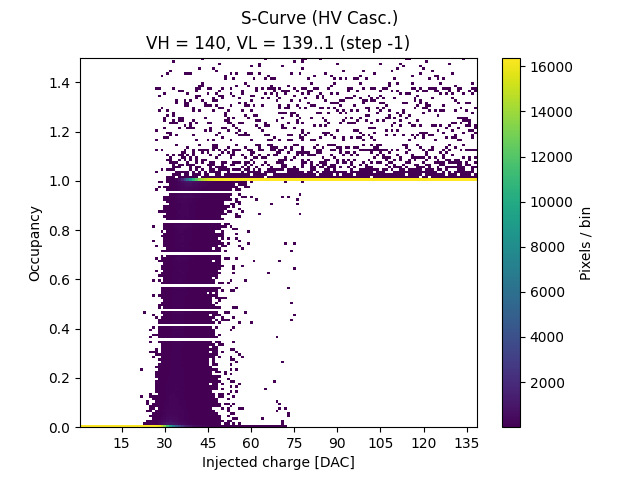
\includegraphics[scale=.5]{all_HVc_thscan_140}
\caption{S-curves of all pixels in \textbf{HV Cascode} flavor with an injection pulse of 140 DAC.}
\label{fig:hvc_scurve_140}
\end{figure}

In figure \vref{fig:thdist_hvc} are shown the fit of the threshold distribution.

\begin{figure}[h!]
\centering
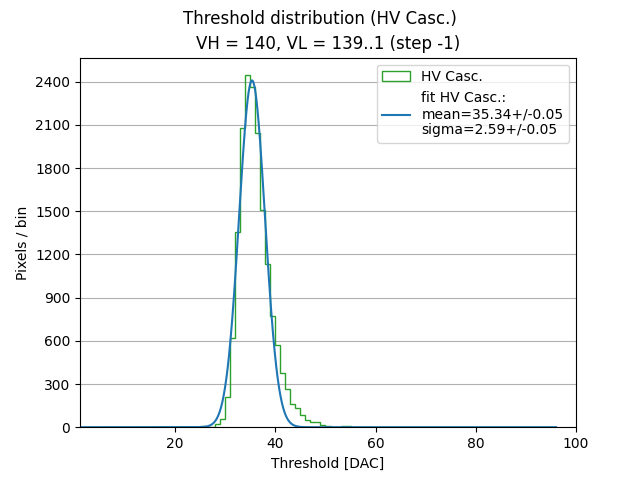
\includegraphics[scale=0.5]{all_HVc_thdist_140}
\caption{Threshold distributions of \textbf{HV Cascode} flavor for VH = 140 DAC.}
\label{fig:thdist_hvc}
\end{figure}


\subsubsection{HV-Normal FE}

The fourth and last flavor is the \textbf{HV-Normal FE} which consists of 512 rows and 32 columns for a total number of pixel equal to 16.384. The main registers have been set with the values reported in table \vpageref{tab:tb_hv_settings}.
In figure \vref{fig:hv_scurve_140}, the S-curves of all pixel in the flavor. Also here we can see that there were some noisy pixels unmasked.
Moreover, in this final flavor, the last 16 columns were not working and as a matter of fact they had return a peak of threshold near the value 0, which is excluded from the threshold distributions plots.

So actually in this part of the matrix, the real number of pixel studied was the half of the total, such as 8192 pixels.


\begin{figure}[h!]
\centering
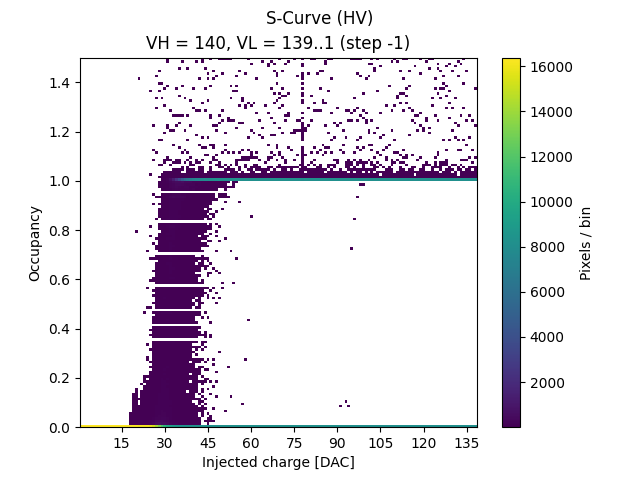
\includegraphics[scale=.5]{all_HV_thscan_140}
\caption{S-curves of all pixels in \textbf{HV Cascode FE} with an injection pulse of 140 DAC.}
\label{fig:hv_scurve_140}
\end{figure}

In figure \vref{fig:thdist_hvc} the fit of the threshold distribution.


\begin{figure}[h!]
\centering
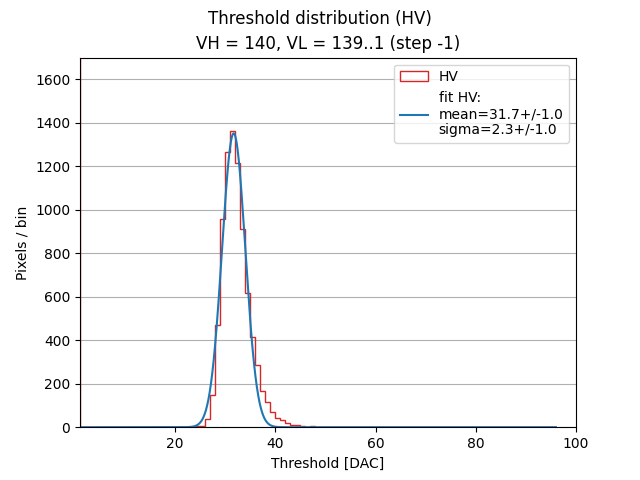
\includegraphics[scale=0.5]{all_HV_thdist_140}
\caption{Threshold distributions of \textbf{HV} flavor for VH = 140 DAC}
\label{fig:thdist_hvc}
\end{figure}


\subsubsection{Summary Table}

\begin{table}[h!]
\centering
\begin{tabular}{>{\columncolor{NavyBlue!70}} c|c|c|c}
\rowcolor{CornflowerBlue}
Front-End & Threshold [$e^{-}$] & Threshold dispersion [$e^{-}$] & Noise [$e^{-}$]\\
\hline
Normal  & 53.62 $\pm$ 0.01 & 2.21 $\pm$ 0.01 &\\
\hline
Cascode & 60.19 $\pm$ 0.01 & 2.81 $\pm$ 0.01 &\\
\hline
HV & 35.34 $\pm$ 0.05 & 2.59 $\pm$ 0.05 &\\
\hline
HV - Cascode & 31.70 $\pm$ 0.10 & 2.30 $\pm$ 0.10 &\\
\hline
\end{tabular}
\caption{Summary table of threshold and noise values for all flavors of the W14R12 chip.}
\label{tab:th_noise_all}
\end{table}





%--------------------------------------------------------------------
\subsection{Threshold dispersion and tuning}
%\subsection{Noise and Equivalent Noise Charge (ENC)}
%%TUNING PAGINA 136 DELLA TESI



IN THE END\\
Results from measurements done later (Ludovico talk TREDI) pre and post




%--------------------------------------------------------------------
\section{ToT calibration with internal injection}




%--------------------------------------------------------------------
\subsection{Injection circuit issues}

In carrying out the measurements mentioned above, we started to noticed some issues with the injection circuit, which seemed to limit its working range. As a matter of fact the height of the injection pulse is expected to grow linearly increasing the value of charge to be injected.
It actually happened up to a value of (about) $\approx$ 140 DAC, but for higher quantities of injected charge, the circuit seemed to increase not only the height of the signal, but also the threshold by a certain amount of $\Delta V$ (or equivalently of $\Delta Q$, related by the conversion factor reported in REFERENCE). Moreover, for injection height grater than 200 DAC, only the threshold grows, without increasing the actual injected charge in any way.\\
We come to the conclusion that the grows of the threshold was artificial and due to the failure of the injection circuit.[?]

However as we have seen in the previous section (reference), the threshold depends on the settings of the chip registers and it can't be influenced by the injected charge, otherwise the whole response of the chip would be chaotic and it would not be reliable to take precise measurement of the impinging particles. 

For this problem, the investigation on the behaviour of the threshold and its dispersion of all flavours of the matrix, required a series of additional measurements.\\
In the following sections the method used to obtain a reliable value of threshold and ToT is explained.

%\subsection{Measurement of the average threshold shift for injected charge greater than 140 DAC}

To evaluate this artificial shift of the threshold, two different measurements have been done for each flavor:

\begin{itemize}
\item for an injected charge equal to 140 DAC $\rightarrow$ before the saturation region;
\item for an injected charge equal to 200 DAC $\rightarrow$ almost the maximum limit of the saturation region (from this value onward only the threshold increases, not the injected charge).
\end{itemize}

The threshold distributions obtained from each measurements have been fitted to extract an average value on the whole flavor. Naming $Q_{th, 140}$ and $Q_{th, 200}$  the threshold obtained from injections of 140 and 200 DAC respectively, the mean shift has been estimated by:

\begin{equation}
\Delta Q = Q_{th,200} - Q_{th,140}
\end{equation}

Eventually, this charge shift has been subtracted from data collected for an injection pulses of 200 DAC, in order to extrapolate the response in ToT of the injected pixels up to a value of 170 DAC.

What has been obtained is reported in the following section, together with a briefly explanation of the method used to evaluate the threshold.



%--------------------------------------------------------------------
\subsection{Time Over Threshold (TOT) curves and fit}
%\addcontentsline{toc}{subsection}{Curve del Time Over Threshold (TOT) e fit}

A side effect of the injection circuit issue is that the response of the chip can not be characterized in a region of charge that usually corresponds to the emission peaks of the radioactive sources available in the laboratory. 
For this reason, a fit of the ToT obtained at the maximum possible injected charge has been done, in order to extrapolate the most probable value of ToT in the main interesting region of charge.

The function chosen for this purpose is:

\begin{equation}
y(x) = a\cdot x +b -\frac{c}{x-t}
\end{equation}

with \textit{a}, \textit{b}, \textit{c} and \textit{t} free parameters.

Actually we know that the ToT distribution starts to grow near the threshold, so a random parameter could be computed in function of the threshold value estimated from the previous measurements, explained in section (reference).

In particular knowing that y($x_{th}$) must be equal to 0, it can be imposed:

\begin{equation}
0 = a\cdot x_{th} + b - \frac{c}{x_{th}-t}  \hspace{.4cm}	\Rightarrow  \hspace{.4cm}	c = x_{th}^{2}\cdot a + x_{th}\cdot (b-a\cdot t) - t\cdot b
\end{equation}

In this way the number of parameters to fit is reduced.

So the same data collected in the previous measurements of thresholds (for VH=200 DAC unit), have been used to fit the ToT curves of all pixels for each frontend.
In table \vref{tab:th_fe} are reported the value of the threshold considered for each frontend to extrapolate the value of the parameter \textit{c}and the results of the fit for all parameters. In figure \vref{fig:tot_fe} the results obtained for all Normal, Cascode and HVs FE.

\begin{table}[h!]
\centering
\begin{tabular}{c|c|c|c|c}
 & \textbf{Normal} & \textbf{Cascode} & \textbf{HV Cascode} & \textbf{HV} \\
\hline
\textit{threshold [DAC unit]} & 53.62 & 60.19 & 35.34 & 31.70 \\
\textit{a} & & & & \\
\textit{b} & & & & \\
\textit{c} & & & & \\
\textit{t} & & & & \\
\end{tabular}
\caption{Threshold and parameters obtained from the fit of ToT curve for each frontend.}
\label{tab:th_fe}
\end{table}

\begin{figure}[h!]
\centering
\subfigure[\textbf{Normal}]
{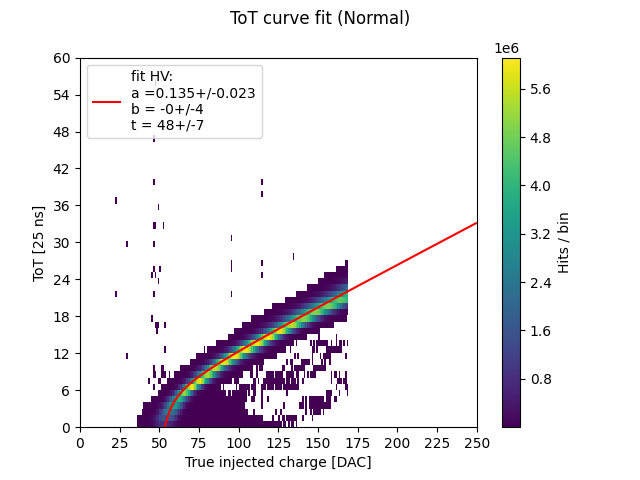
\includegraphics[scale=0.35]{tot_fit_normal(200)}}\quad
\subfigure[\textbf{Cascode}]
{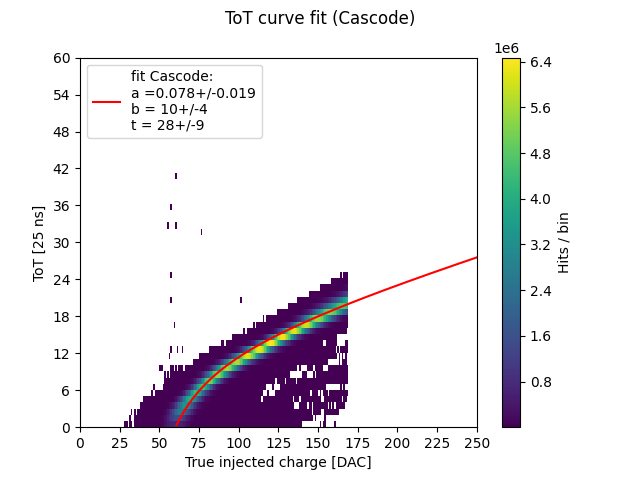
\includegraphics[scale=0.35]{tot_fit_cascode(200)}}\\
\subfigure[\textbf{HV Cascode}]
{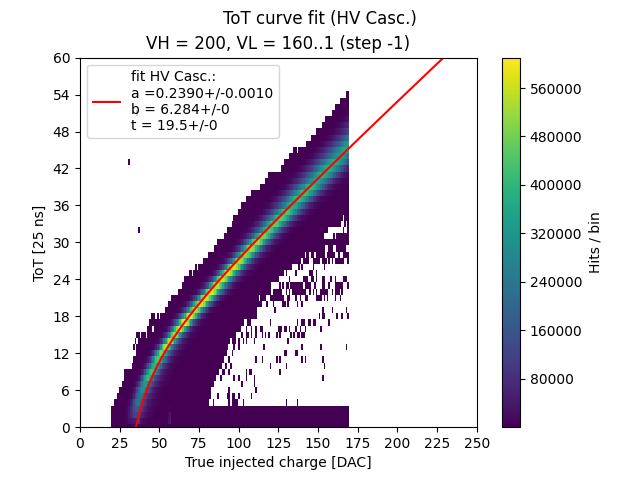
\includegraphics[scale=0.35]{tot_fit_HV_Casc.(200)}}\quad
\subfigure[\textbf{HV}]
{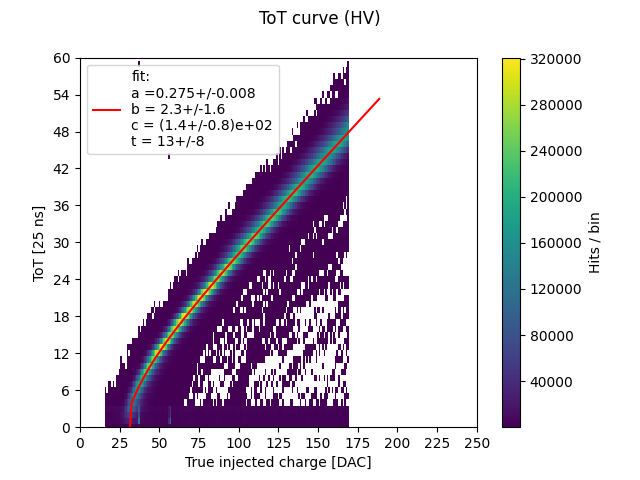
\includegraphics[scale=0.35]{tot_fit_HV(200)}}\\
\caption{ToT curves fit for all frontend.}
\label{fig:tot_fe}
\end{figure}



%--------------------------------------------------------------------
\section{Response to radioactive source and absolute calibration}

%%%%%PAG 55 DELLA TESI PER LA DESCRIZIONE DELLE SORGENTI E FENOMENO


%--------------------------------------------------------------------
\subsection{\ch{^{55}Fe}}

\begin{figure}[h!]
\centering
\subfigure[\textbf{Normal}]
{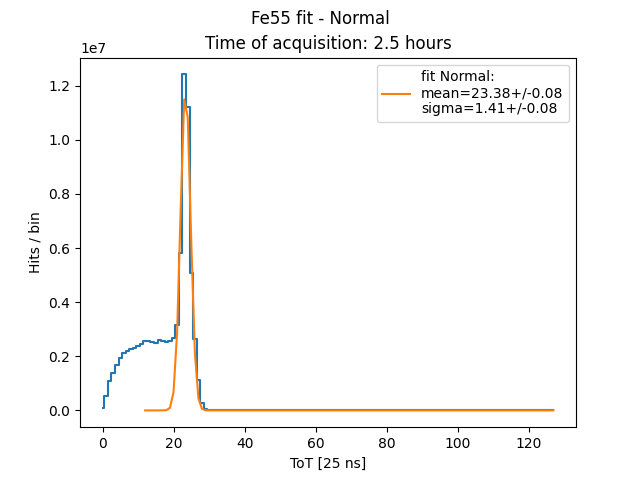
\includegraphics[scale=0.35]{fe55_Normal_peak}}\quad
\subfigure[\textbf{Cascode}]
{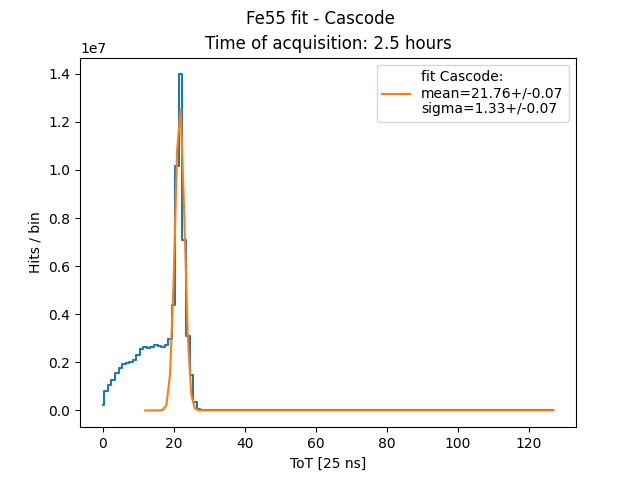
\includegraphics[scale=0.35]{fe55_Cascode_peak}}\\
\subfigure[\textbf{HV Cascode}]
{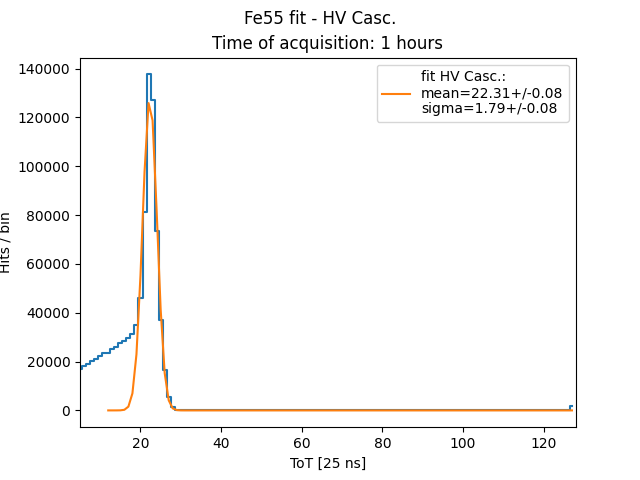
\includegraphics[scale=0.35]{fe_HV Casc._peak}}\quad
\subfigure[\textbf{HV}]
{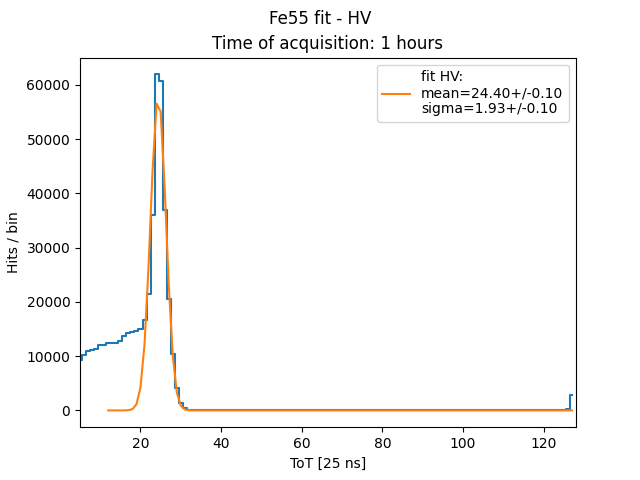
\includegraphics[scale=0.35]{fe_HV_peak}}\\
\caption{\ch{^{55}Fe} pekas for all frontends.}
\label{fig:fe_all}
\end{figure}


CUT ON HVs flavors because of bad columns, many 0 ToT.

%--------------------------------------------------------------------
\subsection{\ch{^{241}Am}}


\begin{figure}[h!]
\centering
\subfigure[\textbf{Normal}]
{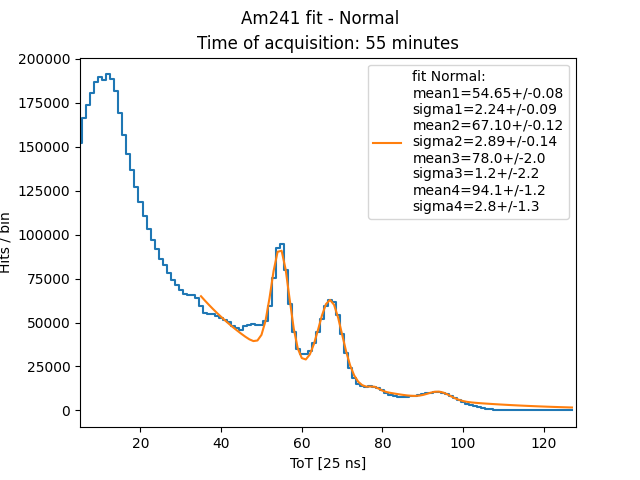
\includegraphics[scale=0.35]{am_Normal_peak}}\quad
\subfigure[\textbf{Cascode}]
{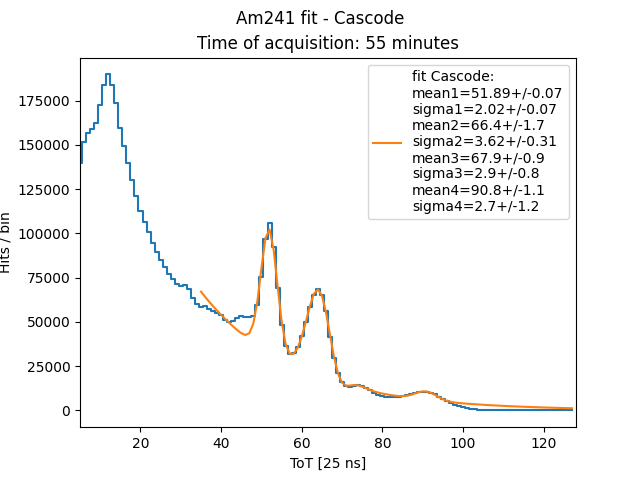
\includegraphics[scale=0.35]{am_Cascode_peak}}\\
\subfigure[\textbf{HV Cascode}]
{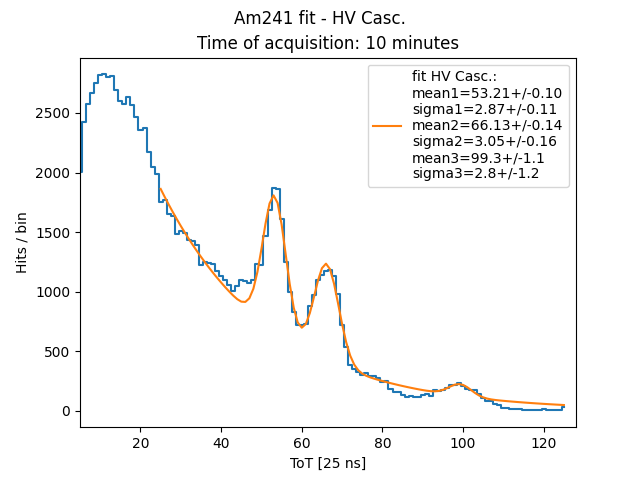
\includegraphics[scale=0.35]{am_HV Casc._peak}}\quad
\subfigure[\textbf{HV}]
{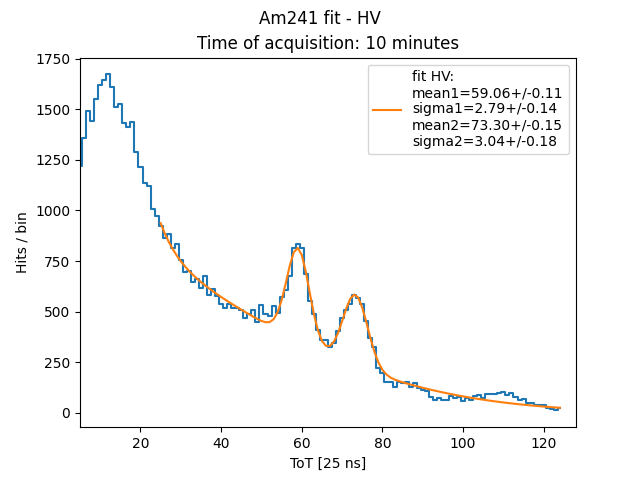
\includegraphics[scale=0.35]{am_HV_peak}}\\
\caption{\ch{^{241}Am} pekas for all frontends.}
\label{fig:fe_all}
\end{figure}

%--------------------------------------------------------------------
\subsection{\ch{^{109}Cd}}

\begin{figure}[h!]
\centering
\subfigure[\textbf{Normal}]
{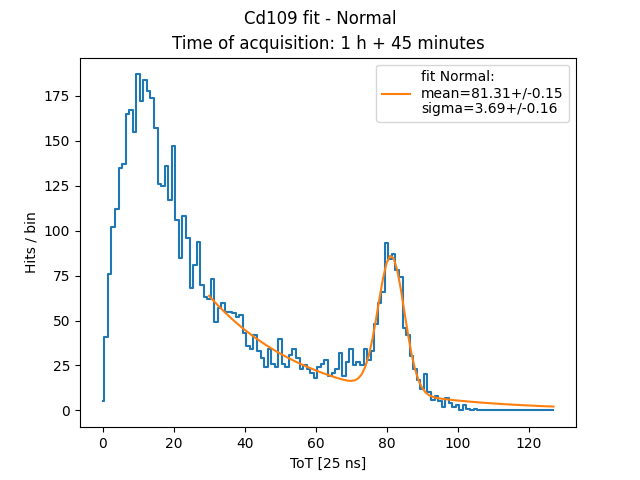
\includegraphics[scale=0.35]{cd109_Normal_peak}}\quad
\subfigure[\textbf{Cascode}]
{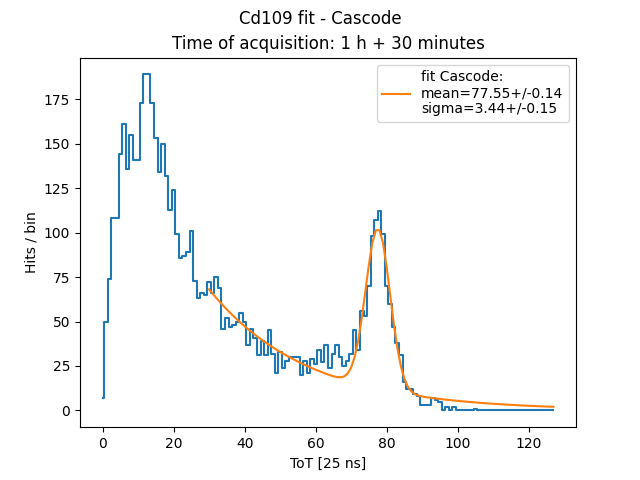
\includegraphics[scale=0.35]{cd109_Cascode_peak}}\\
\subfigure[\textbf{HV Cascode}]
{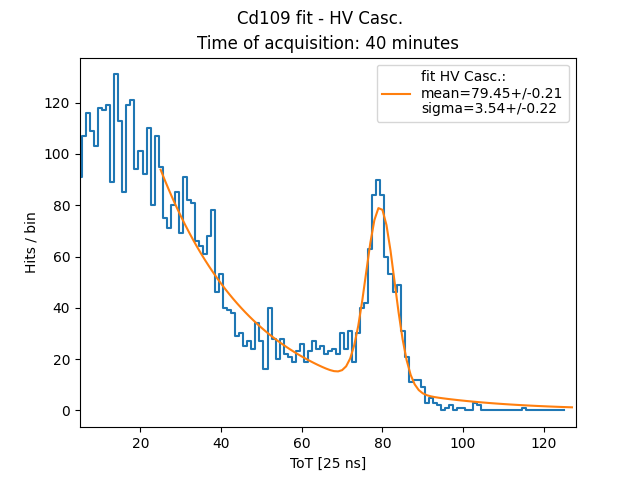
\includegraphics[scale=0.35]{cd109_HV Casc._peak}}\quad
\subfigure[\textbf{HV}]
{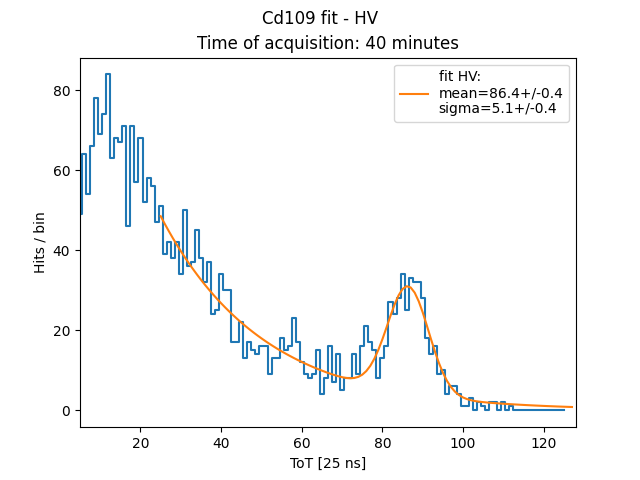
\includegraphics[scale=0.35]{cd109_HV_peak}}\\
\caption{\ch{^{109}Cd} pekas for all frontends.}
\label{fig:fe_all}
\end{figure}

%--------------------------------------------------------------------
%\subsection{\ch{^{190}Sr}}

\subsection{Injection capacitance calibration}
%\addcontentsline{toc}{subsection}{Calibrazione della capacità di iniezione}



%--------------------------------------------------------------------
\section{Operation with low threshold}
%\subsection{Mask (operation) and noisy pixels}
%\subsubsection{Main registers (and conversion?)}

%% VOGLIAMO OPERARE A BASSE THRESHOLD PER IREVARE EVENTI A BASSE CARICA A CAUSA DEL CHARGE TRAPPING AND CHARGE SHARING SOPRATTUTTO IN CASO DI THIN EPITAXIAL MATERIAL.

\begin{comment}
Explain the function of the various registers used (see Eleonora thesis, and maybe can 		add also some scope picture). 
	Register optimization
	Comparison with simulation 
	Can add at the end some nice picture of the optimized thr and tuning 
\end{comment}


%--------------------------------------------------------------------
\subsection{Register optimization}



%--------------------------------------------------------------------
\subsection{Comparison between data and simulation}
%\addcontentsline{toc}{subsection}{Confronto degli andamenti con le simulazioni}

In the interest of understanding how the settings of the chip influence the threshold's value, several measurements have been taken varying the values of the main registers which are responsible for it.
The results are compared with simulations done by Hung Pham (...). [???]

\subsubsection{$I_{CASN}$}

This current is responsible of the output baseline. In a few words, higher this value, higher the baseline, lower the threshold and also a little bit the gain.

In figure \vref{fig:icasn_sim}, we can see the simulated behaviour of the threshold and the gain, increasing the value o $I_{CASN}$.

\begin{figure}[h!]
\centering
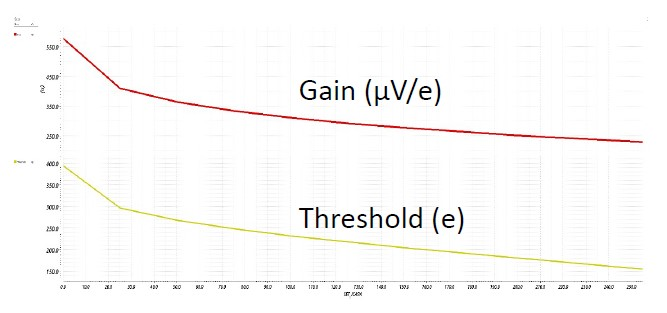
\includegraphics[scale=.9]{thr_gain_icasn(sim)}
\caption{Trends of Gain and Threshold increasing $I_{CASN}$.}
\label{fig:icasn_sim}
\end{figure}

To verify the trend of threshold in particular, three different acquisition have been taken by fixing $I_{THR}$ = 20, 40, 64 and increasing $I_{CASN}$ from 0  to 30 DAC, with a step of 5 DAC. We have done this enabling 200 pixels in the Cascode FE (rows: 472 - 512, cols: 225 - 230).[??]\\

The threshold distributions have been fitted with a gaussian function for each measurement,  in order to obtain the average values and their dispersion.

\begin{itemize}
\item[$I_{THR}=64$]:

\begin{tabular}{c | c | c}
$I_{CASN}$ [DAC] & THR [DAC] & THR Dispersion [DAC]\\
\hline
0 & 61.43 & 2.45\\
5 & 53.42 & 2.45\\
10 & 50.33 & 2.45\\
15 & 48.21 & 2.41\\
20 & 46.70 & 2.38\\
25 & 45.49 & 2.52\\
30 & 46.09 & 2.50
\end{tabular}

\item[$I_{THR}=40$]:

\begin{tabular}{c | c | c}
$I_{CASN}$ [DAC] & THR [DAC] & THR Dispersion [DAC]\\
\hline
0 & 47.28 & 2.12\\
5 & 41.07 & 2.02\\
10 & 38.39 & 2.03\\
15 & 36.65 & 1.95\\
20 & 35.53 & 1.91\\
25 & NaN & NaN\\
30 & 33.37 & 2.04
\end{tabular}

[Here we can see a particular setting, that is $I_{THR}=40$ AND $I_{CASN}$=25, for which the chip doesn't seem to work.
PIXEL THAT FIRE UP??]

\item[$I_{THR}=20$]:

\begin{tabular}{c | c | c}
$I_{CASN}$ [DAC] & THR [DAC] & THR Dispersion [DAC]\\
\hline
0 & 34.43 & 1.95\\
5 & 28.10& 1.72\\
10 & 26.59 & 1.75\\
15 & 24.66 & 1.77\\
\end{tabular}
\medskip\\

\end{itemize}

In figure \vref{fig:alltrends_icasn} all trends obtained from these data are reported.

[TREND OF DISPERSION?]

\begin{figure}[h!]
\centering
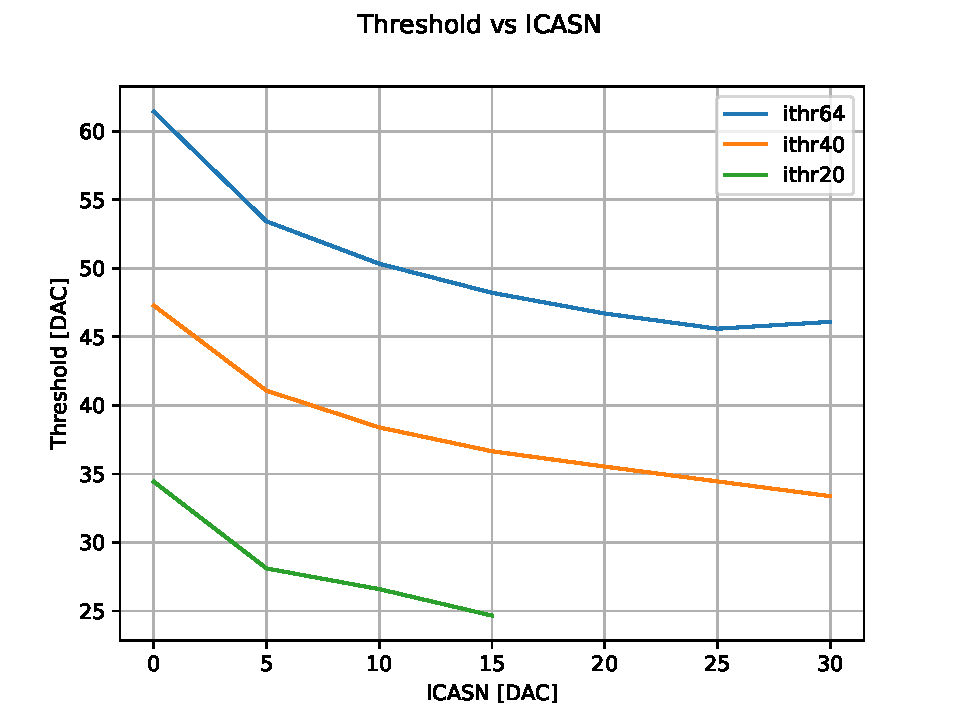
\includegraphics[scale=.7]{all_trends(ICASN)}
\caption{Threshold vs. $I_{CASN}$ for $I_{THR}$= 20, 40, 64.}
\label{fig:alltrends_icasn}
\end{figure}

\subsubsection{$I_{THR}$}

Reusing the same data of the previous measurements, the trend of the threshold have been studied, changing the value of $I_{THR}$ and fixing that of $I_{CASN}$. In this case only $I_{CASN}$ from 0 to 15 DAC is considered, because for higher values we don't have enough measures of the threshold (specifically only two for $I_{THR}$=40, 64). The results are shown in figure \vref{fig:alltrends_ithr}.

\begin{figure}[h!]
\centering
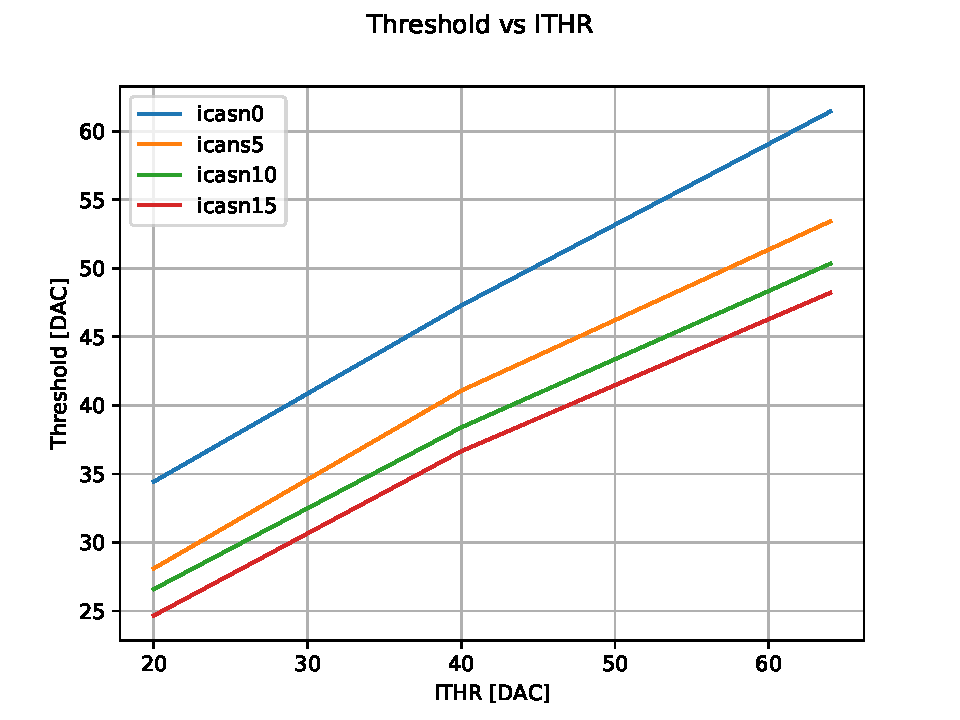
\includegraphics[scale=.7]{all_trends(ITHR)}
\caption{Threshold vs. $I_{THR}$ for $I_{CASN}$= 0, 5, 10, 15.}
\label{fig:alltrends_ithr}
\end{figure}

We can compare them with the simulation done by Hung Pham in figure \vref{fig:ithr_sim}. 

\begin{figure}[h!]
\centering
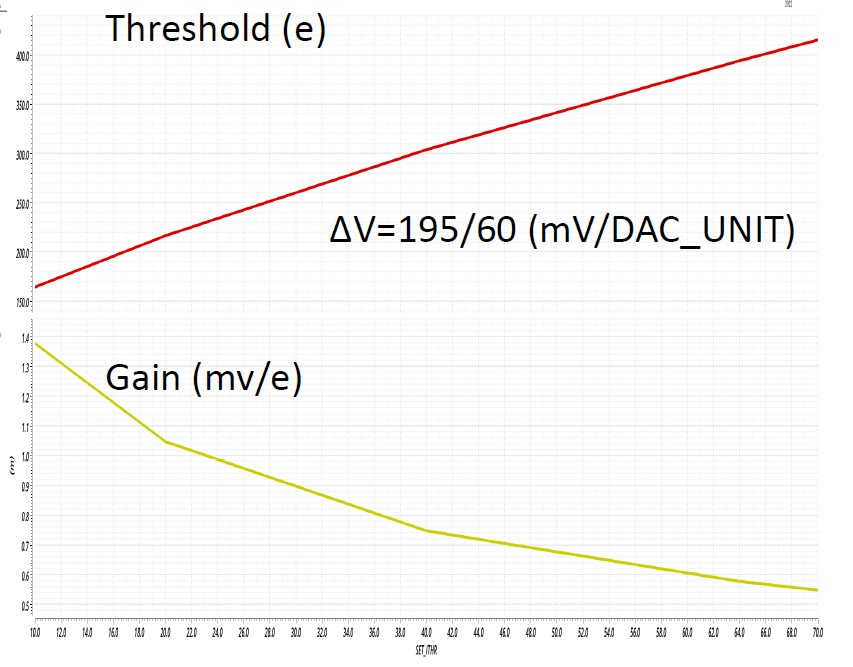
\includegraphics[scale=.7]{ithr_simulation}
\caption{Trends of Gain and Threshold increasing $I_{CASN}$.}
\label{fig:ithr_sim}
\end{figure}



\subsubsection{Time over Threshold (ToT)}

The last analysis done in order to make a comparison with the simulations, is about the trend of the ToT changing the value of $I_{CASN}$ for a fixed value of $I_{THR}$ and vice versa. In particular we consider the data obtained with $I_{CASN}$ fixed to 0 DAC and $I_{THR}$ to 64 DAC, which are the values studied and used for this registers during the Test Beam in Desy.

\begin{figure}[h!]
\centering
\subfigure[ToT vs $I_{THR}$ ($I_{CASN}$=0 DAC) - Data (\textbf{Cascode})]
{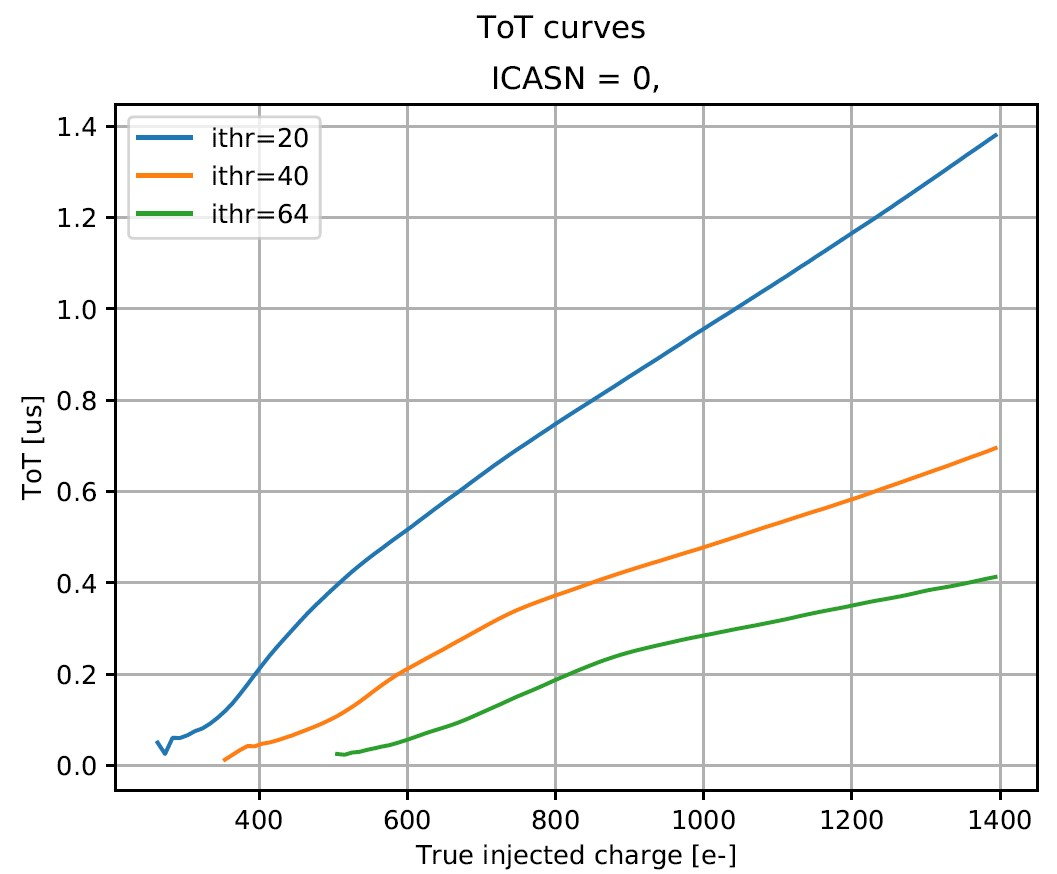
\includegraphics[scale=0.5]{tot_curves_icasn0}}\quad
\subfigure[ToT vs $I_{THR}$ ($I_{CASN}$=0 DAC) - Simulation]
{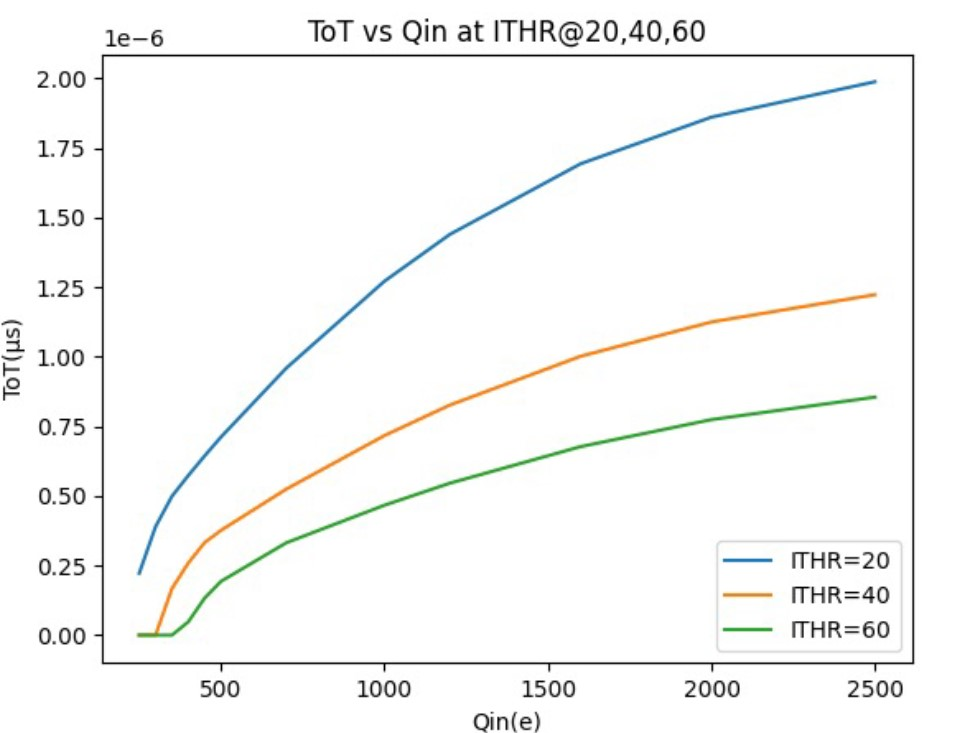
\includegraphics[scale=0.4]{tot_curves_icasn0_simu}}\\
\caption{ToT vs $I_{THR}$}
\label{fig:tot_vs_ithr}
\end{figure}

\begin{figure}[h!]
\centering
\subfigure[ToT vs $I_{CASN}$ ($I_{THR}$=64 DAC) - Data (\textbf{Cascode})]
{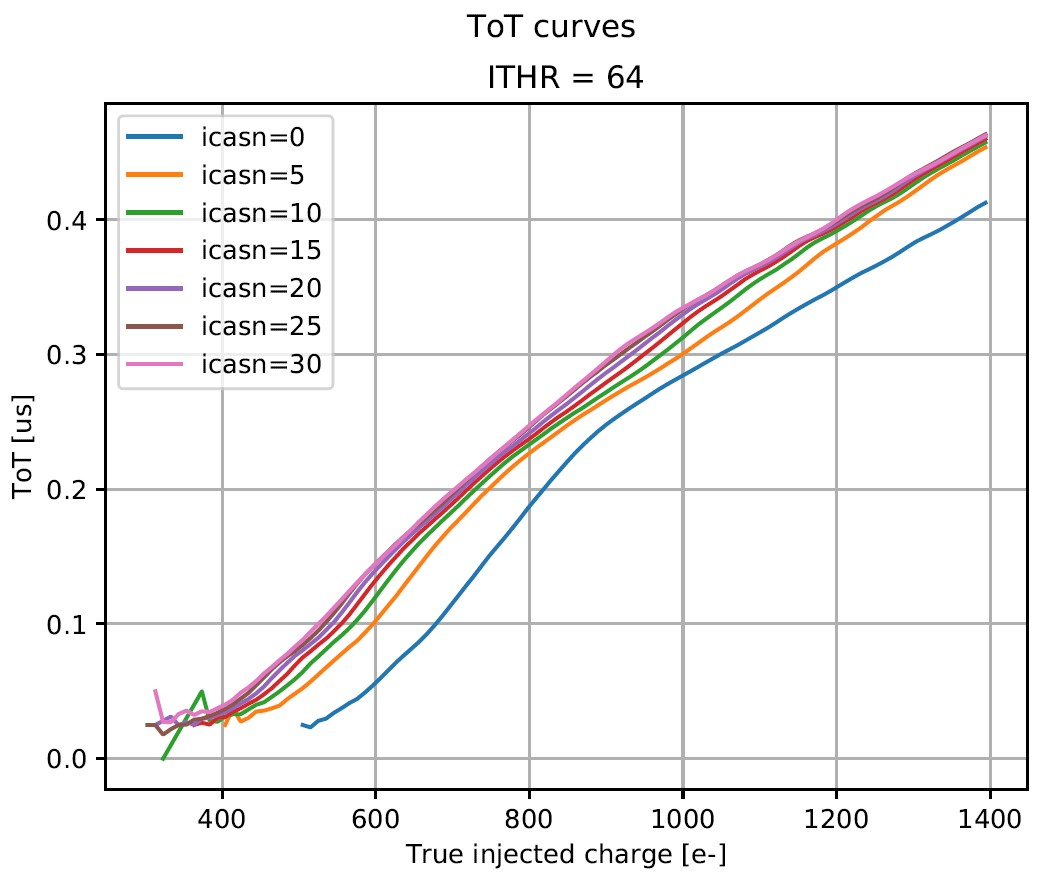
\includegraphics[scale=0.5]{tot_curves_ithr64}}\\%\quad
\subfigure[ToT vs $I_{CASN}$ ($I_{THR}$=64 DAC) - Simulation]
{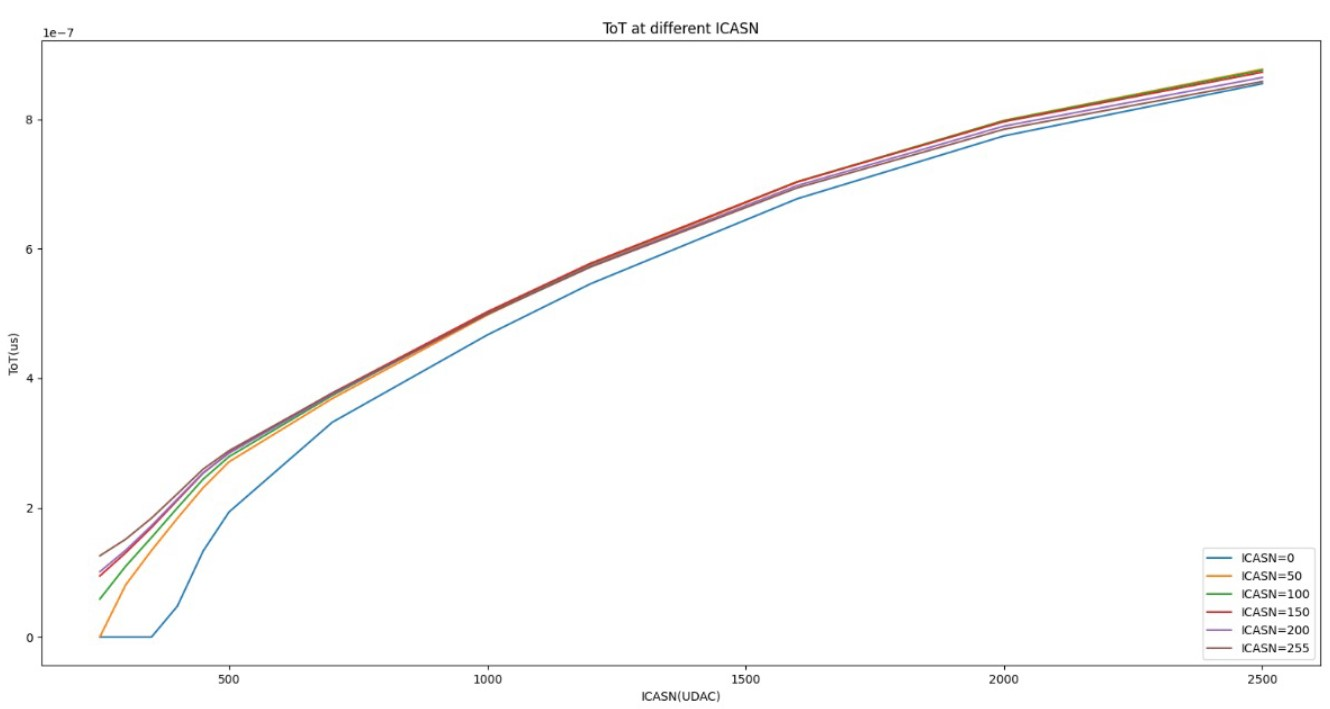
\includegraphics[scale=0.35]{tot_curves_ithr64_simu}}\\
\caption{ToT vs $I_{CASN}$}
\label{fig:tot_vs_icasn}
\end{figure}


\begin{comment}
In the last plots of this section (\vpageref{fig:tot_vs_vcasp}) are reported the trends of the ToT varying the value of $V_{CASP}$ for both Normal and Cascode FE, but there aren't simulations to make a comparison. 

\begin{figure}[h!]
\centering
\subfigure[ToT vs $V_{CASP}$ - Data (\textbf{Cascode})]
{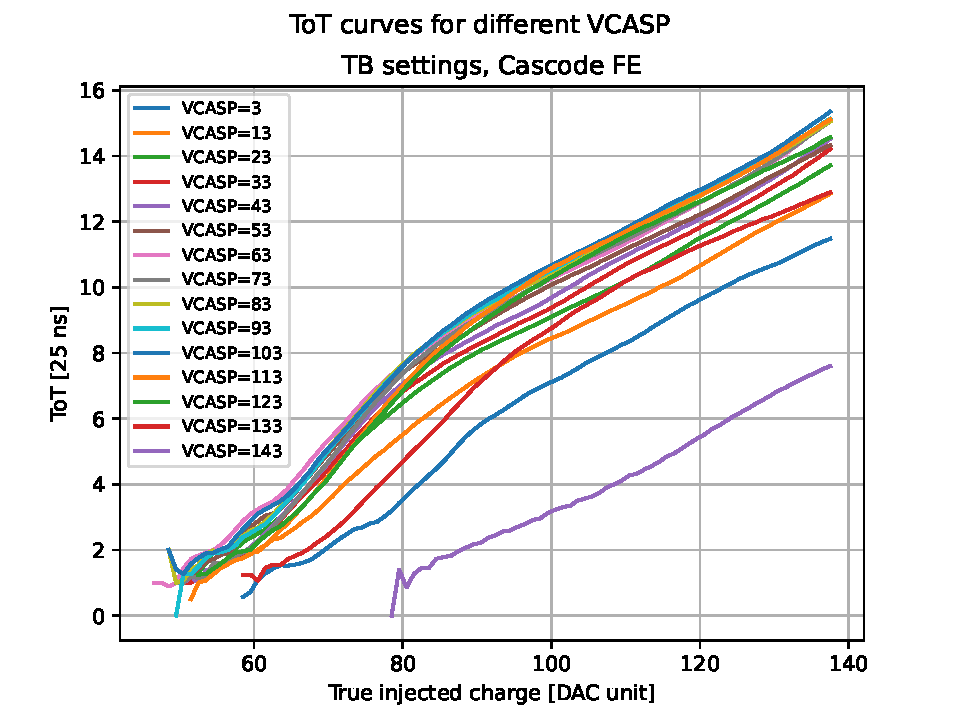
\includegraphics[scale=0.4]{tot_vcasp(cascode)}}\quad
\subfigure[ToT vs $V_{CASP}$ - Data (\textbf{Normal})]
{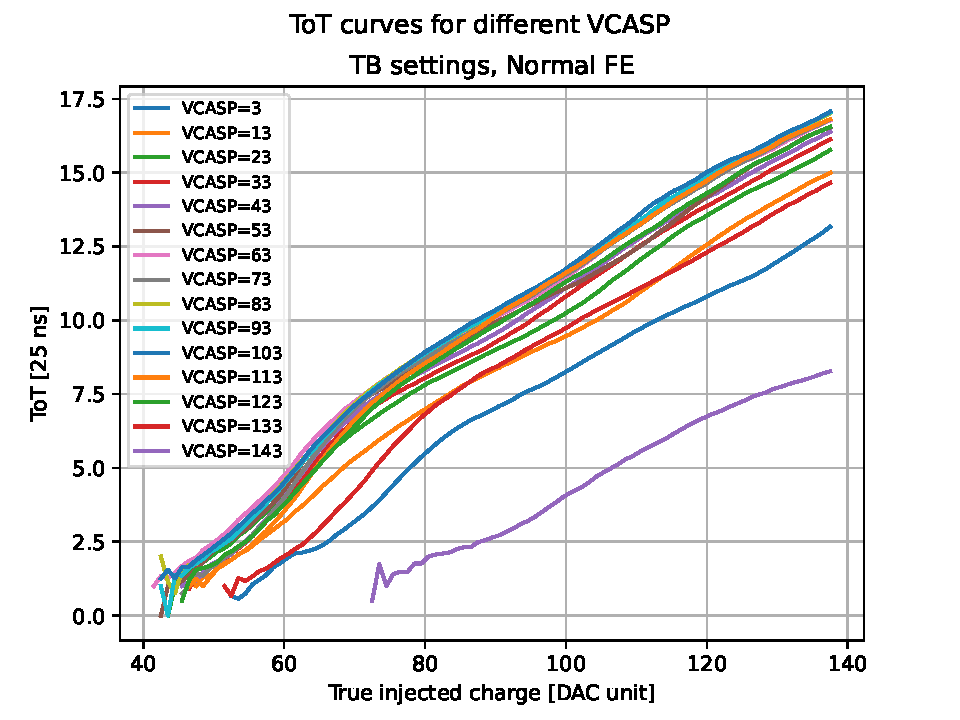
\includegraphics[scale=0.4]{tot_vcasp(normal)}}\\
\caption{ToT vs $V_{CASP}$}
\label{fig:tot_vs_vcasp}
\end{figure}
\end{comment}



\section{Cross talk issue and mitigation}

\section{Test Beam results}






%\subsection{Analog and digital readout}   %Alla fine del quarto??

%\subsubsection{BCID reset}




%%%%%%%%%%%%%%%%%%%%%%%%%%%%%%
%			COMMENT						
%%%%%%%%%%%%%%%%%%%%%%%%%%%%%%


\begin{comment}
In the prototype under test (the chip W14R12), some problems had come up right from the beginning, for both the analog and digital part of the pixel readout.
Despite its predecessor Tj-Monopix 1, Tj-Monopix 2 is equipped with a circuit which allows the \textit{threshold tuning}. In other words it can adjust every pixel threshold, even if only by few DAC, in order to have a global threshold on the matrix as uniform as possible, or in any case a dispersion as small as possible.
\end{comment}

\begin{comment}
\subsubsection{$V_{CASP}$}

[Explain VCASP]

In order to enhance this type of analysis, other scans have been run increasing the value of $V_{CASP}$ from 3 to 143, with a step of 10 DAC unit. In figure \vref{fig:th_vs_casp} the threshold's trend with respect to different values of this register.

\begin{figure}[h!]
\centering
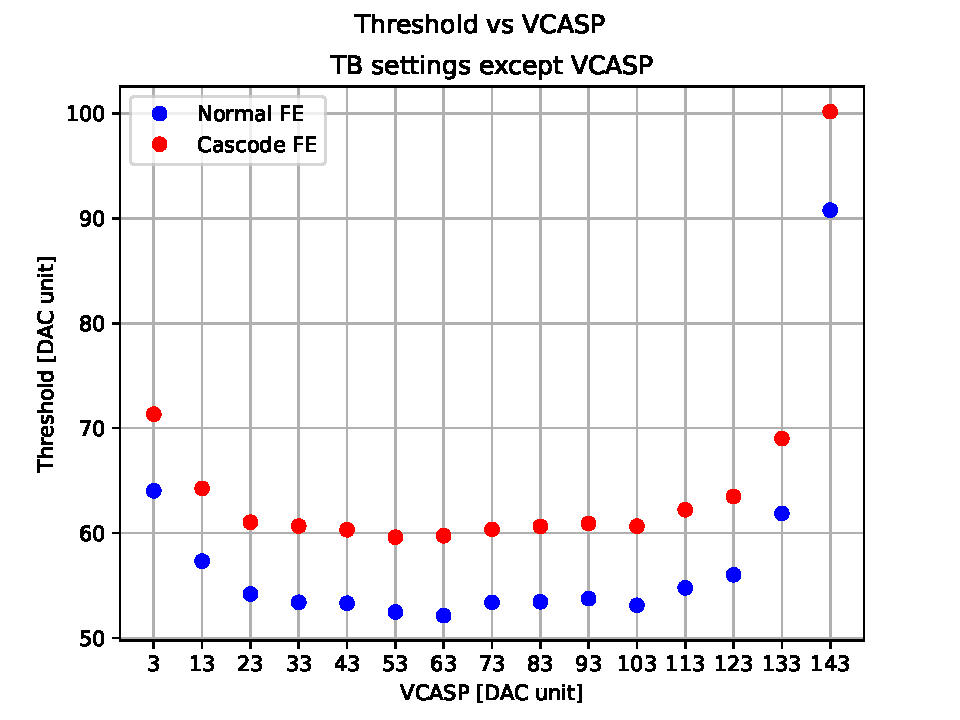
\includegraphics[scale=.7]{TH_vs_VCASP(point)}
\caption{Trends of Threshold increasing $V_{CASP}$.}
\label{fig:th_vs_casp}
\end{figure}
\end{comment}


\begin{comment}
\begin{figure}[h!]
\centering
\subfigure[VH = 140 DAC]
{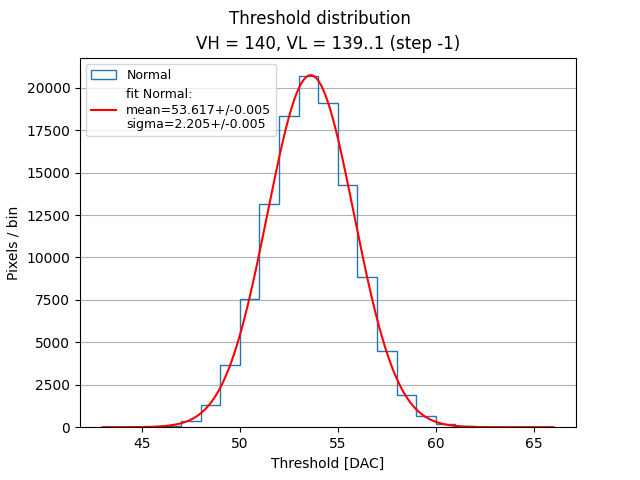
\includegraphics[scale=0.6]{all_norm_thdist_140}}\quad
\subfigure[VH = 200 DAC]
{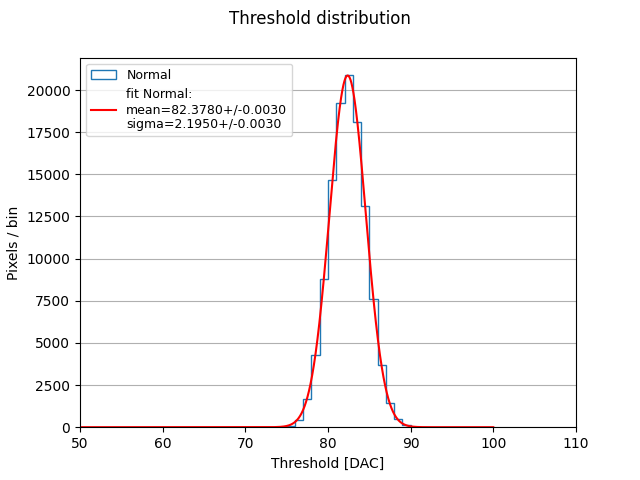
\includegraphics[scale=0.6]{all_norm_thdist_200}}\\
\caption{Threshold distributions of \textbf{Normal} flavor before and at the maximum saturation, respectively.}
\label{fig:thdist_norm}
\end{figure}

\begin{figure}[h!]
\centering
\subfigure[VH = 140 DAC]
{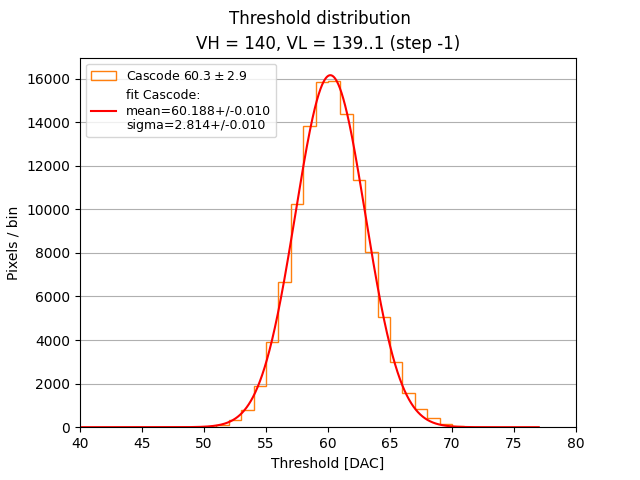
\includegraphics[scale=0.5]{all_casc_thdist_140}}\quad
\subfigure[VH = 200 DAC]
{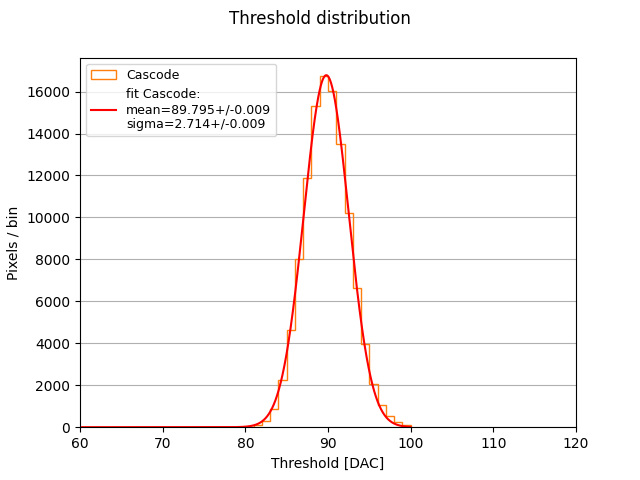
\includegraphics[scale=0.5]{all_casc_thdist_200}}\\
\caption{Threshold distributions of \textbf{Cascode} flavor before and at the maximum saturation, respectively.}
\label{fig:thdist_casc}
\end{figure}

\begin{figure}[h!]
\centering
\subfigure[VH = 140 DAC]
{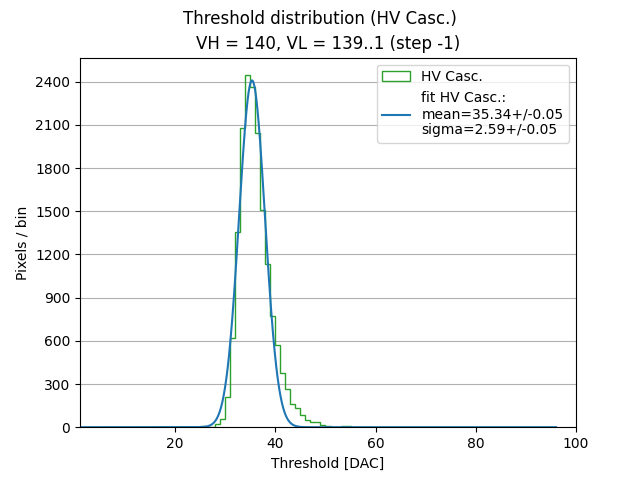
\includegraphics[scale=0.5]{all_HVc_thdist_140}}\quad
\subfigure[VH = 200 DAC]
{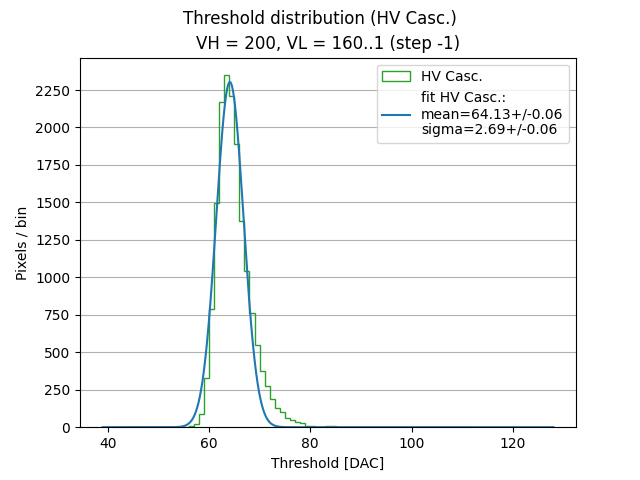
\includegraphics[scale=0.5]{all_HVc_thdist_200}}\\
\caption{Threshold distributions of \textbf{HV Cascode} flavor before and at the maximum saturation, respectively.}
\label{fig:thdist_hvc}
\end{figure}

\begin{figure}[h!]
\centering
\subfigure[VH = 140 DAC]
{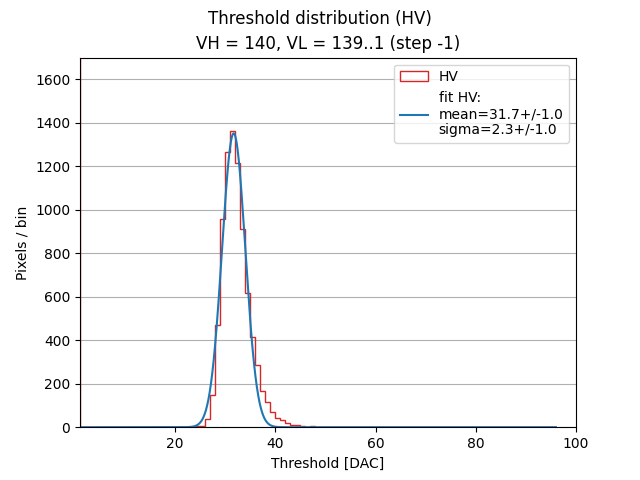
\includegraphics[scale=0.5]{all_HV_thdist_140}}\quad
\subfigure[VH = 200 DAC]
{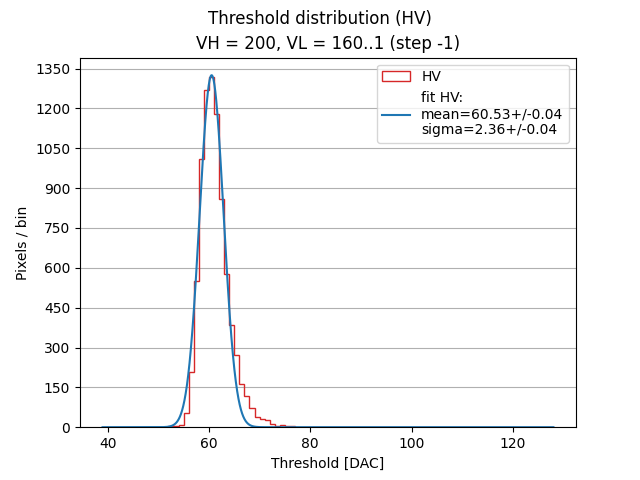
\includegraphics[scale=0.5]{all_HV_thdist_200}}\\
\caption{Threshold distributions of \textbf{HV} flavor before and at the maximum saturation, respectively.}
\label{fig:thdist_hvc}
\end{figure}
\end{comment}

%------------------------------------------------------------

\begin{comment}
TB SETTINGS
SCRIVI DA TESI MUST

NO 

The ultimate purpose of this measurement is to describe (characterize) the response of each pixel by injecting a charge equivalent to the typical energy released from particles emitted in decays of radioactive materials. As explained in the previous section (reference), for example the \ch{^{55}Fe} has an emission spectrum with quite sharp lines and this allows to compare data more easily. The first line is at 5.9 KeV which corresponds on average to about 1616 $e^{-}$ released (through the pixel??).
For this reason it's mandatory to know the conversion between DAC and $e^{-}$ [reference?] and to inject charges in order to study the pixel behaviour in the right regions, so those which are more interesting from a physical point of view.

Preliminarly it was necessary to study the threshold distribution on the whole matrix. The four flavors have been separately analyzed to be able to study their main difference concerning their performance and features.

\begin{figure}[h!]
\centering
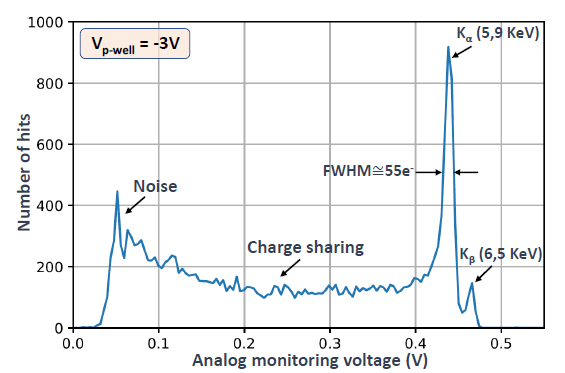
\includegraphics[scale=0.8]{spectrum_fe}
\caption{\ch{^{55}Fe} (radiactive source) emission spectrum using the analog output of a PMOS reset front-end of TJ-Monopix 1. (reference)}
\label{fig:fespectrum}
\end{figure}

\end{comment}

\begin{comment}
For the greater (higher) injection height, 8 different measurement have be actually done, each one on 28 consecutive columns and on all rows. Then data have been put together to obtain a single (summary) plot on the whole flavor. Same procedure has been preformed on the \textbf{Cascode FE}.
\end{comment}



%%%%%%%%%%%%%%%%%%%%%%%%%%
%			BIBLIOGRPAHY
%%%%%%%%%%%%%%%%%%%%%%%%%%

%1. THESIS MUSTAKAS
